\chapter{Structure of online supportive conversations}
\label{chap:structure_support}

% **************************** Define Graphics Path **************************

\graphicspath{{Chapter4/plots/}}

\section{Introduction}

The world has become more connected over the past decades thanks to the networked nature of the technologies of the day. It is seldom possible to spend a whole day without single interaction on the Internet. The Internet gives platforms where we can not only connect with our social counterparts but also exchange ideas and express opinions. These new mediums have become so ubiquitous, that some research suggests that they might be affecting our broader psychological state \cite{d20122}. But on the positive side, studies have also proposed different ways in which this medium could be used for measuring and intervening in the matters of mental health\cite{DeChoudhury2016,DeChoudhury2014}.
Online communities, or fora, offer a platform for users to directly interact with each other. Reddit\footnote{\url{http://reddit.com/}} is one of the largest online communities which contains a number of sub-communities (so called \emph{subreddits}) that can be about almost anything. On this platform, several subreddits are specifically tailored to mental health-related topics, such as \emph{depression}, \emph{anxiety} or \emph{alcoholism}. These fora offer a unique opportunity to study the way people describe or discuss their problems in their own voice.

One of the most challenging, and devastating, global mental health concerns is suicide. Suicidal behaviour includes any thoughts, plans or acts someone makes towards ending their life. In health care services, preventing death by suicide is a priority, but accurately predicting whether or not someone is at risk of committing suicide is difficult. Moreover, a large proportion of deaths by suicide occur in populations that have never been seen by health service providers.\note{you could probably improve the section above...}

Several online platforms are used for expressing suicidal thoughts and reaching out for support. On Reddit, the subreddit \emph{SuicideWatch} currently\footnote{As of 27th June 2018} has almost 94k subscribers, and is a moderated forum that is intended to offer peer support for people at risk of, or are worried about others', suicidal behaviour. The moderators take the message of peer support seriously, and are governed by guidelines that prohibits false promises, abuse, tough love and other clinically frowned upon methods of conversations\footnote{\url{http://www.bbc.co.uk/newsbeat/article/35577626/social-media-and-suicide-what-its-like-being-a-moderator-on-rsuicidewatch} }

As such it is valuable to understand what characteristics supportive communities like SuicideWatch have, and in what aspects such communities are similar or dis-similar from other casual subreddit conversations. 

%\st{Also given that several of these subreddits that deal with mental health have been studied and proven to help\footnote{https://gizmodo.com/reddit-is-helping-some-people-deal-with-their-mental-he-1825364592}} \cite{Kavuluru:2016:CHC:2975167.2975170,park2018examining}, \st{it is important to dissect and characterize these online conversation threads to understand major differences in terms of structure.}
%\remSVi{Another relevant paper mentioned in the gizmodo piece: \cite{info:doi/10.2196/jmir.8219}}
Recent studies have shown promising results in modeling and measuring signals and patterns in reddit communities related to mental health. For instance, statistical relations of mental health and depression communities with suicidal ideation have been studied \cite{DeChoudhury2014,DeChoudhury2016}. The authors explored linguistic and social characteristics that evaluate user's propensity to suicidal ideation. Approaches to classify reddit posts as related to certain mental health conditions have also been successfully developed, showing that there are certain characteristics specific to mental health-related topics in posts that can be automatically captured\cite{gkotsis2017characterisation}. Furthermore, in a study focused on reddit posts related to anxiety, depression and post-traumatic stress disorder, the authors show that these online communities exhibit themes of supportive nature, e.g. gratitude for receiving emotional support\cite{park2018examining}. Positive effects in participation in such fora have also been shown by improvements in members' written communication\cite{info:doi/10.2196/jmir.8219}. The supportive nature of comments in the SuicideWatch forum has also been studied by automatic identification and classification of helpful comments with promising results\cite{Kavuluru:2016:CHC:2975167.2975170}.


%\st{One aspect of this is measuring} \sv{measure} signals and patterns in the data that are predictors of certain distresses. A good example\cite{DeChoudhury2014,DeChoudhury2016} looked at statistical relations of mental health and depression community with suicidal ideation. In their work, the authors explore linguistic and social characteristics that evaluate user's propensity to suicidal ideation. 
%Another crucial and related work was carried out by \cite{gkotsis2017characterisation}, where they characterized mental health related posts on sub-reddit, and developed models to accurately predict type of condition based of informed language models.

Most previous studies have aimed at studying the \emph{content} of posts and their characteristics in relation to other posts. One important aspect of online communities is its supportive \emph{function} --- users turn to these platforms not only to express their thoughts and concerns, but also to receive support from the community. 
\note{More references to be added in the introduction. Also, we need to add something about the Online disinhibition effect somehow.}

To our knowledge, there are no studies that have specifically focused on modeling the supportive \emph{nature} of online fora related to mental health. This work takes a macroscopic perspective, to quantitatively characterise and model the nature of supportive conversations. SuicideWatch is particularly interesting because of its purpose to offer peer support to people with suicidal thoughts, and also because of the complexity of this clinical construct.

Our aims in this study are to 
\begin{itemize} 
    \item Understand similarities and differences between a Suicide watch conversation and a generic conversation using these abstraction. 
    \item Study global properties of these conversations in comparison with control conversations. 
    \item User network metrics to reason about global differences in terms of local interactions between users. 
\end{itemize}

% 1) understand the nature of the posts and replies that are posted in this forum from a clinical perspective, and 2) study the supportive nature of the forum on a global level. We do this by 1) performing a qualitative analysis of a random subset of posts [this needs to be explained somehow], 2) Develop a method of representing conversations on these forums in a computationally measurable format and 3) operationalizing a theory of community support\cite{minkler2005improving} in a data-driven approach using network topology and content feature approaches, and comparing these against a control dataset.

To model the network topology in an online community, we represent conversations in a forum using graph-based abstractions (users and replies) as described in Section \ref{Sec:Abstractions}. 
To measure global structure of these conversations, we user network topological metrics such as centrality: which measures importance of nodes in a network in terms of relaying information, branching factor: which measures how a conversation fans our over time, return distance: which measures how soon do users return back to the conversation and symmetric edges: which measures reciprocity of users in a conversation. To measure measure local interactions, we measure inter response times: which measure urgency of response to a message, semantic alignment between messages and local interaction motifs known as Triadic motifs : which gives an idea about how distinctive are interactions between subgroups of users. 

%We propose a set of metrics for network topology analysis that capture the supportive nature of online communities like SuicideWatch: thread engagement, response times, symmetric responses, centralities, topical alignment, branching factors, return distance and \sj{local user interaction structure \cite{holland1976local}}. \st{triadic motifs [not sure if we should mention these here - if we do, maybe they need brief introductions/explanations or pointers to the details in the methods section]. This method provides a means to systematically analyze these types of online communities. [We need a sentence on the main contributions too here.]}




\begin{table}
    \resizebox{0.5\linewidth}{!}{
        \begin{tabular}{l|p{8cm}}
            \textbf{Terminology} & \textbf{stands for}\\
            $RP$   & Root post which begins a new thread on a subreddit \\
            $OP$  & Original poster who posts the Root post for a thread \\
            $SW$ & The suicide watch Subreddit \\
            $FP$  & Front page of Reddit. \\
    \end{tabular}}
    \caption{Notations and Terms.}
    \label{notations}
\end{table}

% \st{In this work we measure the phenomenon of social support in online communities that deal with suicidal thoughts and suicidal expressions. We do this by a data driven study of Suicide Watch sub-reddit and baseline it using a large random collection of reddit threads from the Front page of the Reddit website. We in the process of measuring, try to ope rationalize a well establish theory on off-line support from literature \cite{minkler2005improving} using network topology and content features and show that the measures developed off-line hold true for this particular supportive community}


%% SV: to add: condense the punchline and the main methods and contributions. 5 main steps - network structure would be the typical network analysis which actually doesn't show anything in these datasets, but with the subsequent methods proposed here, significant differences are shown, and they provide a means to systematically analyze these types of communities

% This work takes a macroscopic perspective, it shows the nature of supportive conversations. This could be used to find conversations that seem to be supportive and this could be used to study the content of these to better understand - also to automatically create datasets for - precurated - for analysis and annotation of content. How is this useful for someone like Rina? Could this (motifs) be used to inform the design of therapy groups? (Put in discussion) There are certain motif structures that are important in supportive conversation - would this translate to online conversations? 
% this is a way to elicit something that has been done qualitatively previously
% group support online
% follow-up studies: are specific motif structures particularly supportive? 
% real-time graphical display? evolving communication structure that could be used by moderators? how does the moderation work today?



\section{Results}
Particularly Suicide watch community consists of over 78k subscribers and reader, however is supported by mere 12 Moderators according to the latest count. The moderators are mainly present to prevent any kind of abuse, trolling or non-clinical or non-productive advices. These moderators do not have any form of formal training. However through several accounts they have confessed to learn through interactions and mentorship from more senior moderators on the site\footnote{\url{https://bbc.in/24rJYQH}} All the moderators have been in that role for at least 3 years and the oldest goes as far as December 2008. 

Our study is based on all conversations on SuicideWatch.
We represent these conversations through networked abstractions as described in \ref{Sec:Abstractions}.

Through our analysis we find several discriminatory factors among Suicide watch conversations and generic front page conversation. We show that some of these factors are predictive of suicide watch conversations to a very high degree. We also show that certain properties of these conversations can be backed by sociological theories of real life support conversations. 

\subsection{Peculiarity of threads of Support}
We begin by characterizing the two networked abstractions, namely Reply Graphs and Interaction graphs as described in Section \ref{Sec:Abstractions}. 
We do so by first comparing these two abstractions with a baseline control conversation threads using certain macroscopic network properties. 
We first compare the number of unique users per thread. The two communities exhibit considerable difference. SW Sub-Reddit has a median of 5 users per thread and a mean of 6.7 users and BL threads have a median of 25 users and mean of 50 unique users. So this off the bat indicates that Suicide watch conversations are more intimate and involve less participants. Authors tend to participate on a similar level, with a median participation per author of Suicide Watch to be 5 and for baseline conversations to be 3.

\subsubsection{How urgent are user responses?}
Understanding the inter message times can act as a good proxy for the urgency in a conversation. To understand how Suicide watch subreddit users responds to a $OP$ compared to other sub-reddit threads on the frontpage, we calculate differences between the posting times between consecutive messages in a reply graph. Figure \ref{fig:urgency} shows comparison using CDFs of inter-message response times for SW and FP threads. It can be seen that SW $OP$ are responded with the highest urgency amongst the 4, especially compared to either the $OP$ or any other users or sub-reddits. 

\begin{figure}[!ht]
    \centering
    % \hspace*{-5mm}
    \subfloat[]{
        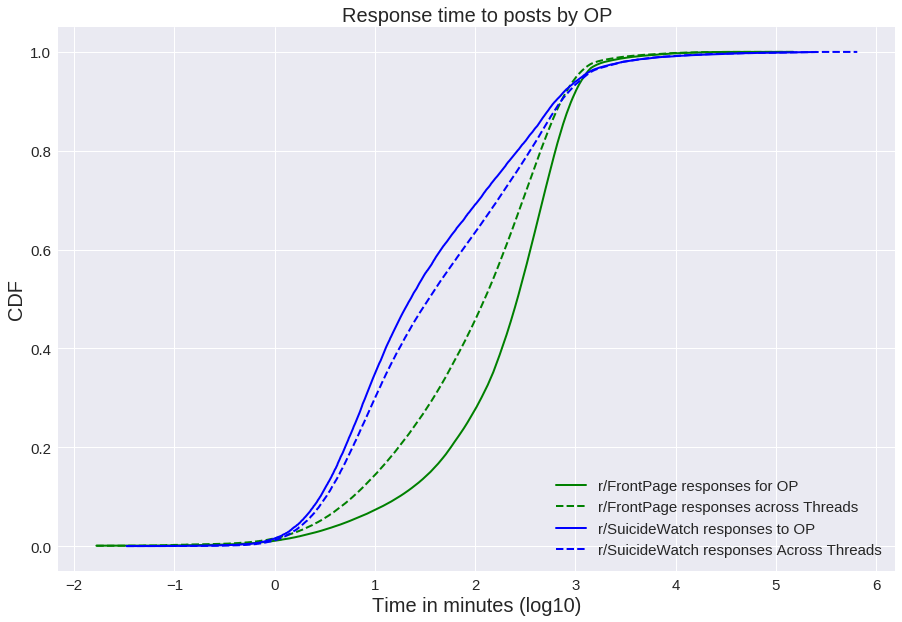
\includegraphics[width=0.4\textwidth ]{respTimeDist.png}
        \label{fig:urgency}
    }
    \subfloat[]{
        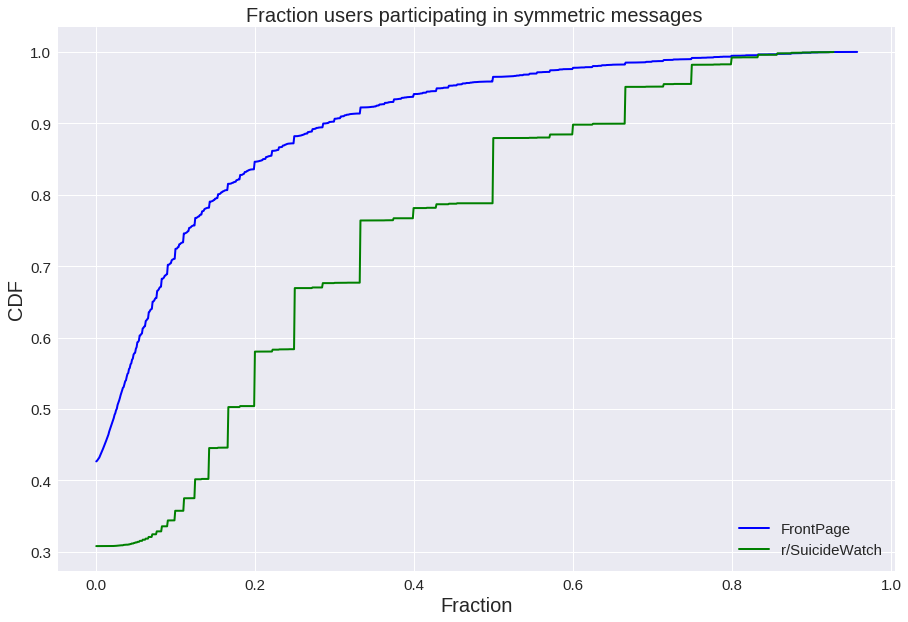
\includegraphics[width=0.4\linewidth ]{SymUsers.png}
        \label{fig:sym}
    }
    
    \subfloat[]{
        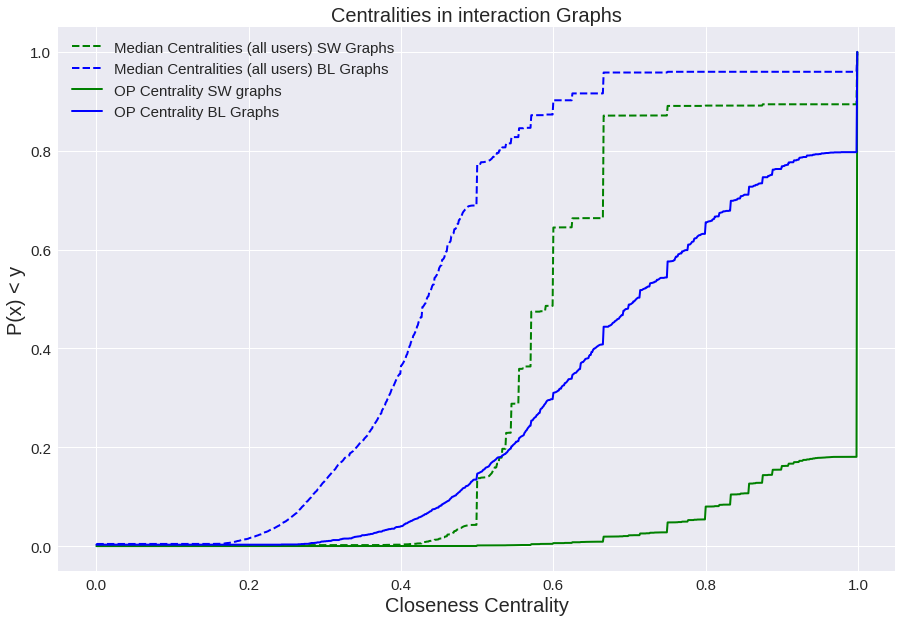
\includegraphics[width=0.4\linewidth ]{AllCentralities.png}
        \label{fig:centrality}
    }
    \subfloat[]{
        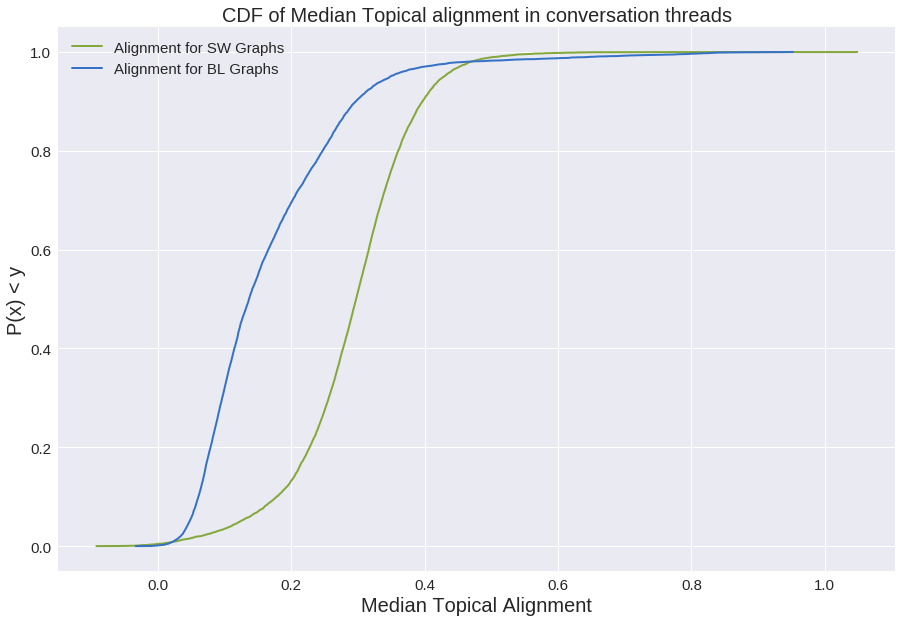
\includegraphics[width=0.4\linewidth ]{medianTA.png}
        \label{fig:topical}
    }
    
    \subfloat[]{
        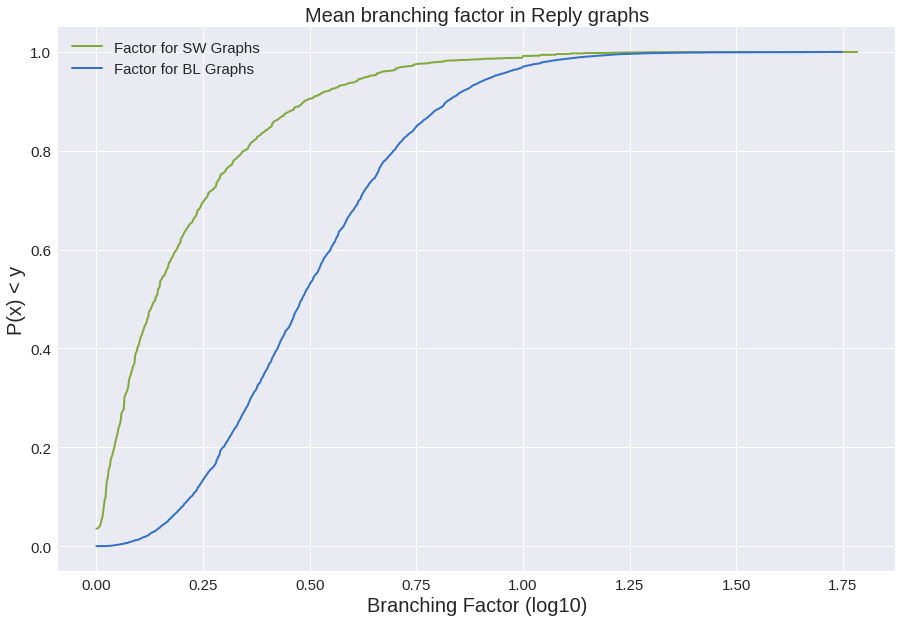
\includegraphics[width=0.4\linewidth ]{meanBranchingFactor.png}
        \label{fig:branching}
    }
    
    
    \caption{Panel shows CDFs of different network metrics. Fig.\ref{fig:urgency} shows the response time distributions, Fig.\ref{fig:sym} shows symmetrically engaged users, Fig.\ref{fig:topical} shows topical similarities across posts and \ref{fig:branching} shows the branching factors of reply graphs. }
\end{figure}

\subsubsection{How symmetric are the interactions?}
Despite signs of urgency and engagement, we ask the question: what percentage of conversations happening on these subreddits are symmetric in nature ? 
For this The median value for $U_{sym}$ for SW is 20\% where as for AS is 0\%. This shows that SW subreddit engages is a lot more symmetric conversation that the baseline threads.
If we define a set of users who engage in symmetric activity with the $OP$ , it would be worth while to investigate how much of the total message activity on the thread is carried out by these set of symmetric users . To calculate this we find the fraction of messages on each thread written as part of this symmetric conversation. Figure \ref{fig:sym} shows the trend. It can be see that SW threads contain a higher prevalence of symmetric message exchanges compared to the baseline Frontpage threads. This shows a higher engagement from the $OP$s side when participating in a supportive conversations

\subsubsection{How central are the users?}
To understand how embedded is the $OP$ in a conversation thread, we compare the betweenness centralities of $OPs$ in the $SW$ dataset with the baseline $FP$ dataset. 
Betweenness centrality is a good proxy of understanding how closely linked is a node with the rest of the network. When we calculate this metric for the user graphs we see that Suicide watch $OP$s tend to have highest centralities compared to generic $FP$ threads moth in terms of $OP$ centrality as well as median centrality across all the users. The high centrality of $OP$s in $SW$ conversations implies a high level of embedded-ness as well as a $OP$ centric approach by other participants in the conversation. The Figure \ref{fig:centrality} shows the Empirical CDFs of centralities. 

\subsubsection{How semantically aligned are the responses?}
We measure semantic alignment based on word embeddings of the source post and the reply post, at every edge of the reply graph. The detailed method of extracting semantic alignment along a post and its response is described in Section \ref{Sec:Semantic}. Extracting such similarity metrics, we compare the trend in response text being in semantic alignment with the parent text in the reply graphs. 


\subsubsection{How branched do conversations become?}
Branching in a conversation thread could be either a sign of digression or a sign interestingness resulting in more people joining in. To measure this phenomena, use the reply graphs, which resemble a n-ary directed acyclic graph, to evaluate the branching factor. By using the method described in Section \ref{Sec:Branching}, we found that Suicide watch threads, tend to branch in a much less as compared to our baseline conversations. This implies that suicide watch threads tend to remain a one-on-one conversation with the $OP$ albeit many such dialogues may emerge, and hence that explains the high centrality of the $OP$ in all interaction graphs. If the helpers on a thread seldom interact with each other, the corresponding interaction graph will have the $OP$ as the most central node.

%\subsubsection{How often do users come back to respond ? }
%This measurement is important as it helps us quantify the average attention of a participant in a conversation, if the participant chooses to remain engaged. 

\subsection{Patterns in local interactions}
It is often a useful tool to express large interaction graphs, as the sum of local interactions between two or three nodes at a time. Such analysis is quite useful in expressing local structures in the graphs and has been used in several network analysis works 
For this reason we use a method more commonly known as network motif analysis (described in Section \ref{Sec:motif}) to understand triads, or groups of three nodes, and the patterns of edges that exist between them. 

\begin{figure*}[!ht]
    \centering
    % \hspace*{-5mm}
    % 	\subfloat[]{
    % 		\includegraphics[width=0.5\textwidth, height = 6cm ]{Figures/RevisedFeatureRegression.png}
    % 		\label{fig:feats}
    % 	}
    % 	\subfloat[]{
    % 		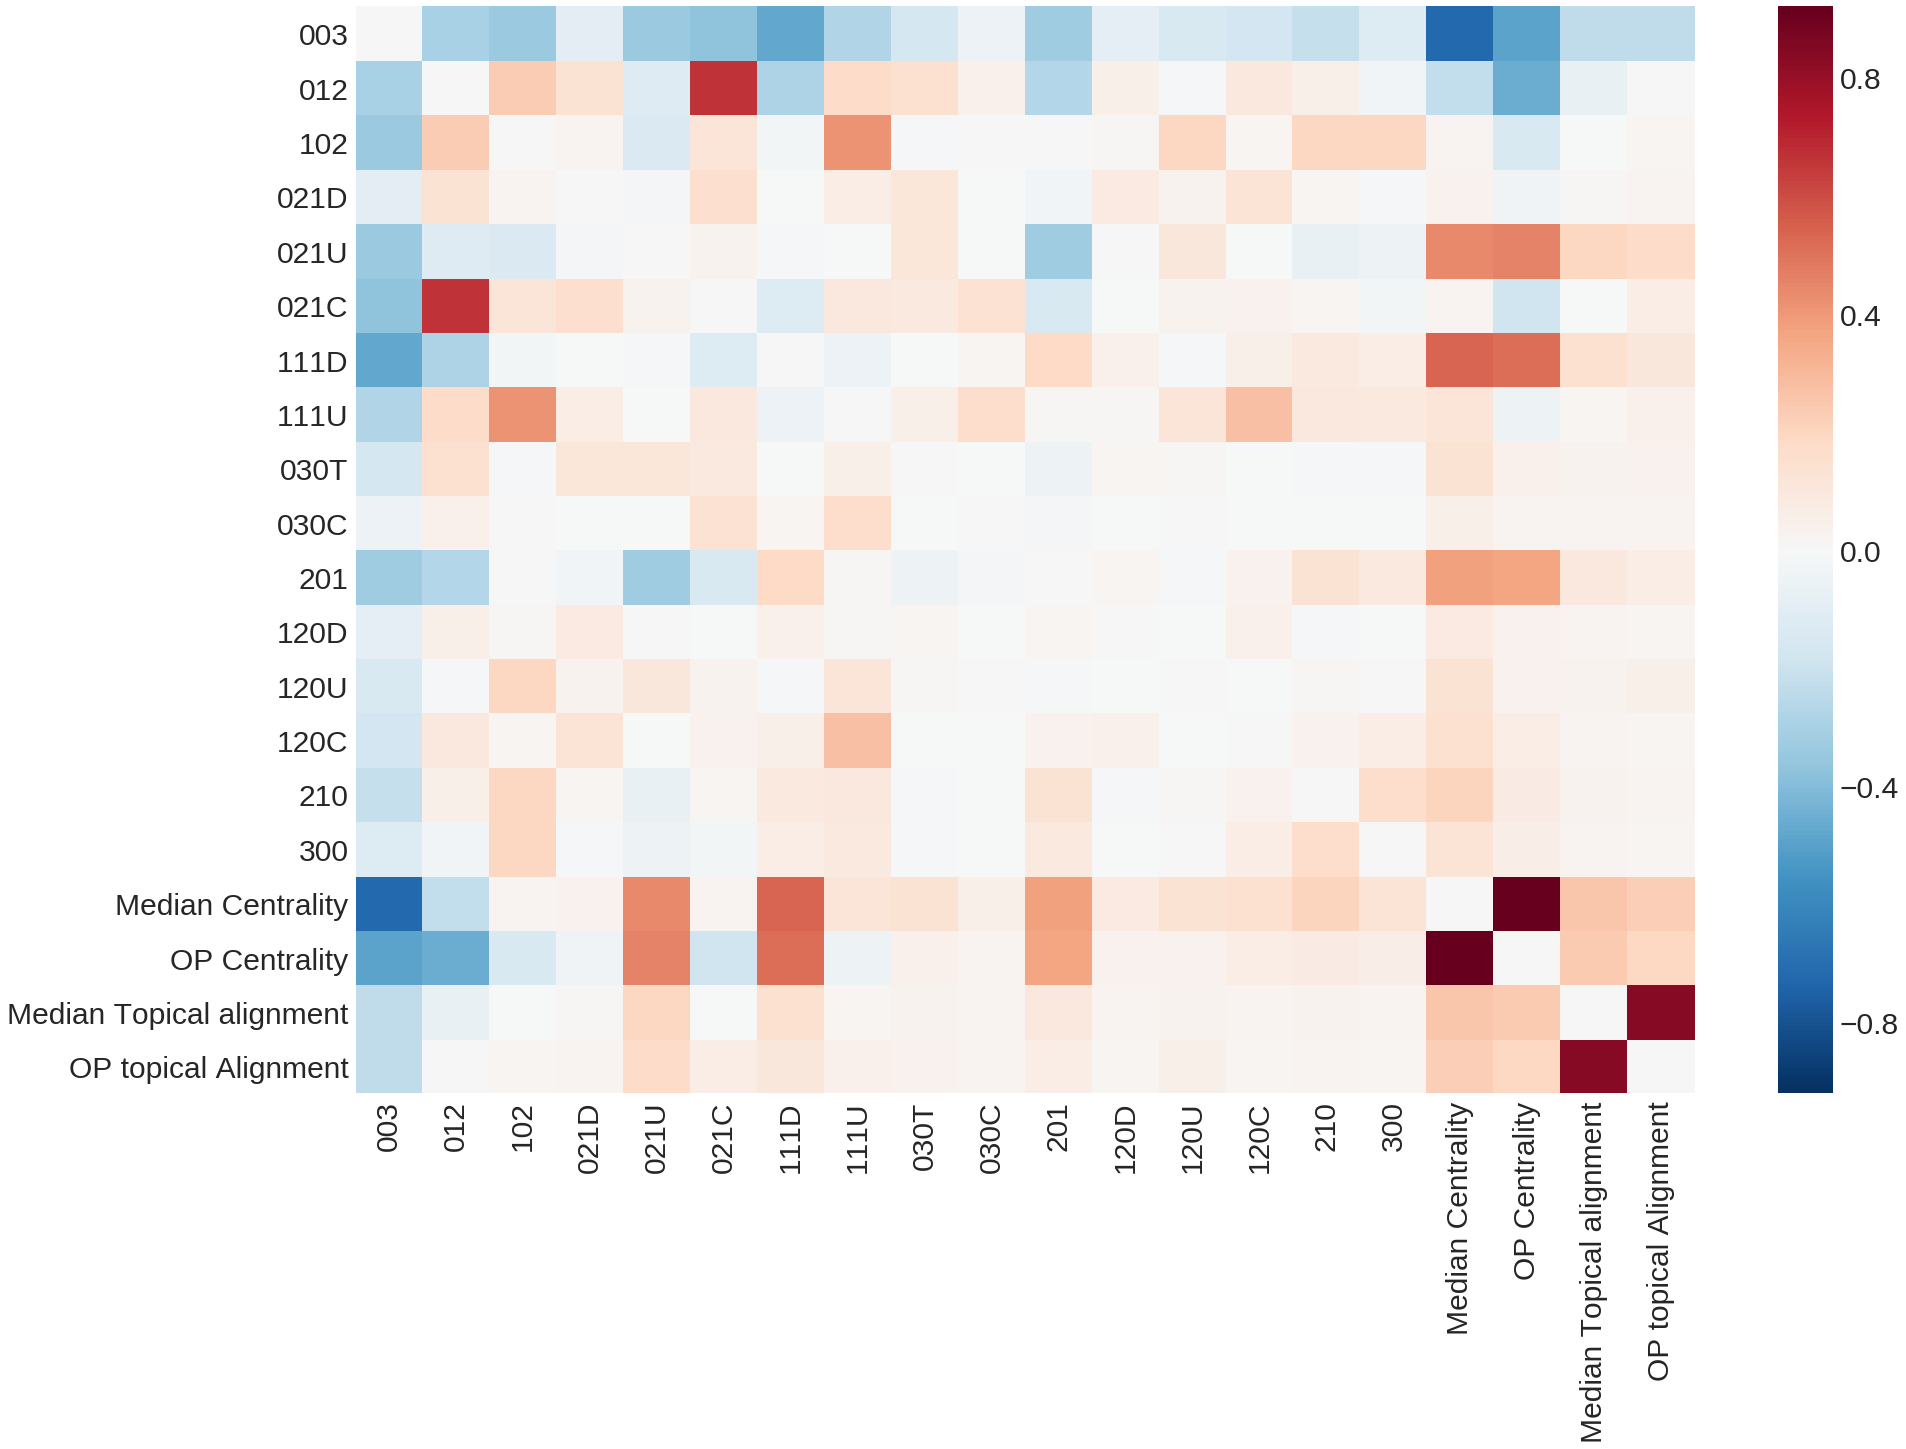
\includegraphics[width=0.5\linewidth, height = 6cm ]{Figures/normalized_corr.png}
    % 		\label{fig:corrs}
    % 	}
    
    \subfloat[]{
        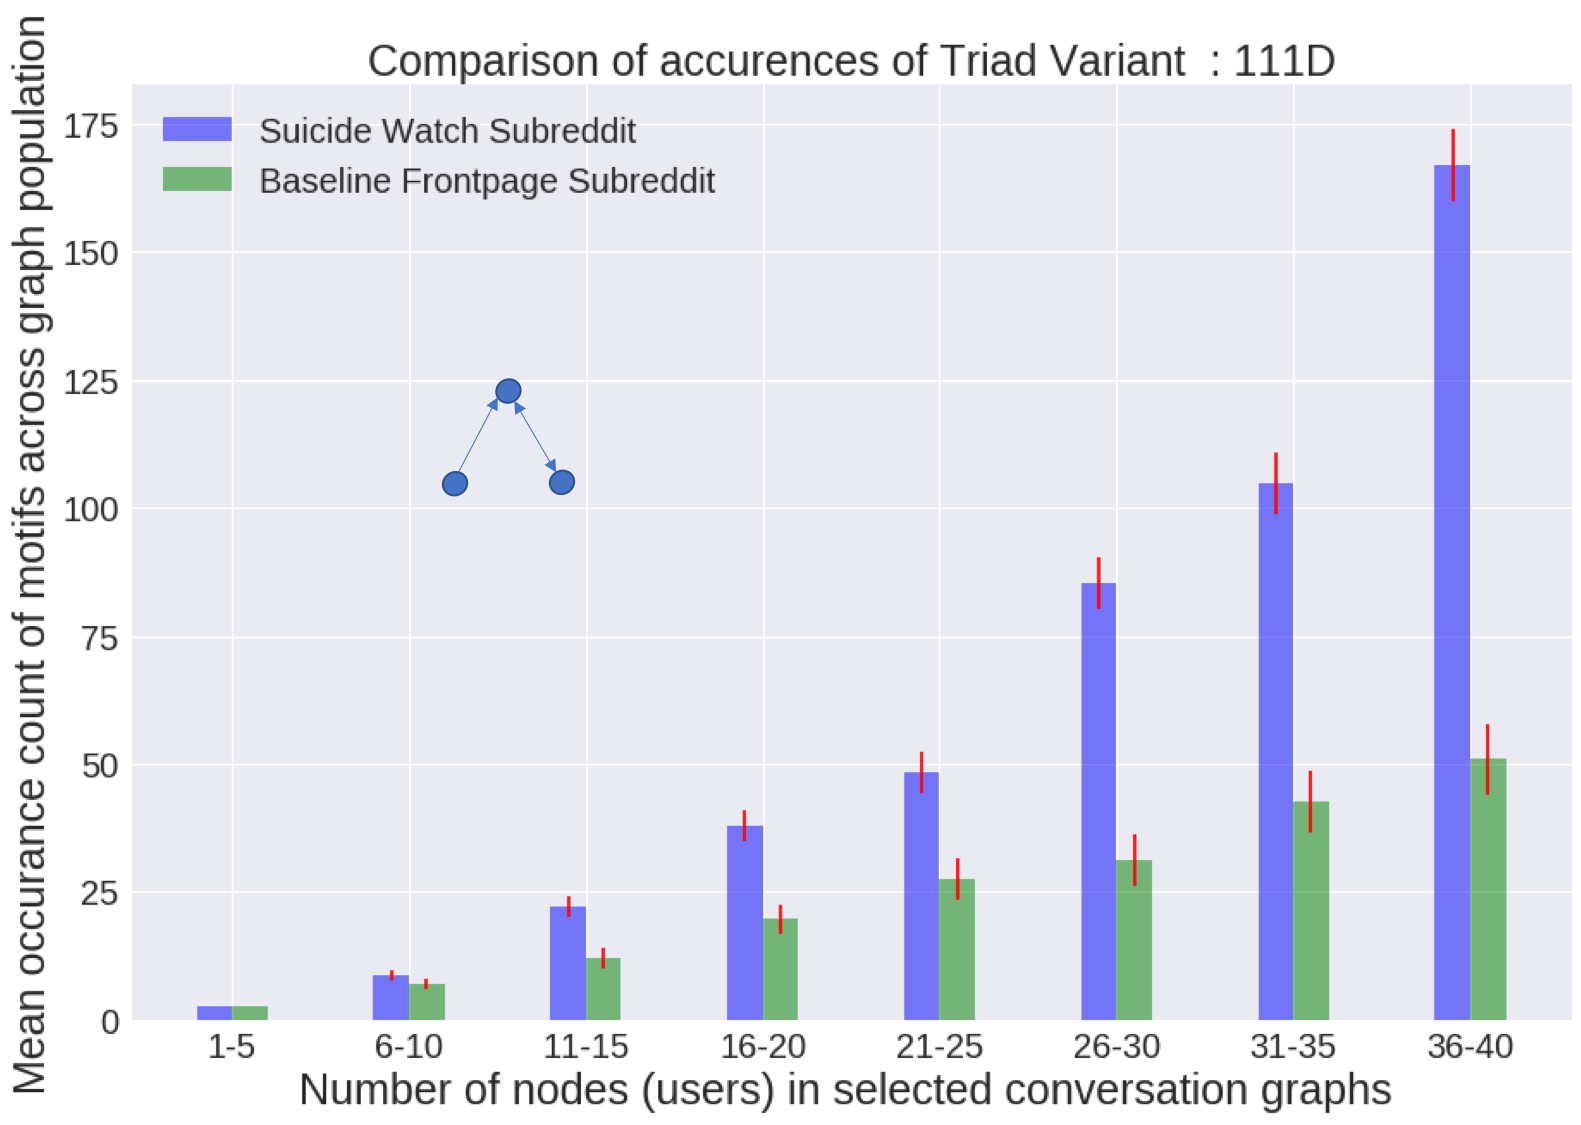
\includegraphics[width=0.5\linewidth ]{111D.png}
        \label{fig:111D_over}
    }
    \subfloat[]{
        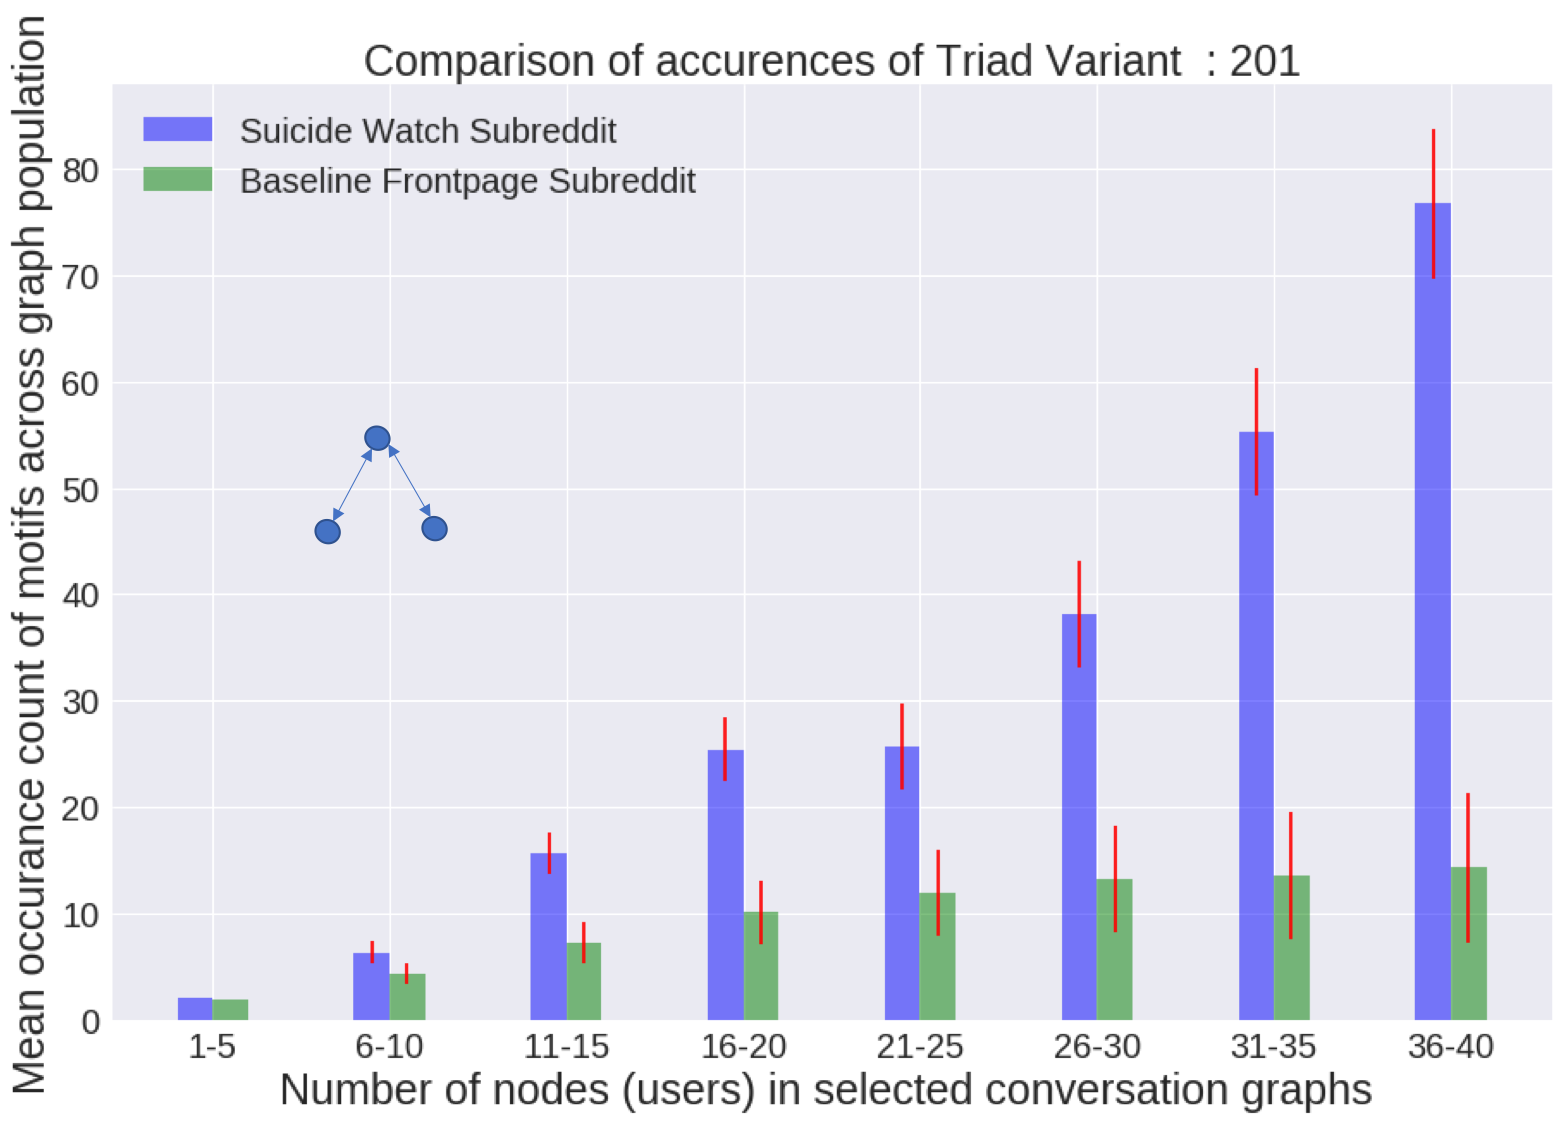
\includegraphics[width=0.5\linewidth ]{201.png}
        \label{fig:201_over}
    }
    
    \subfloat[]{
        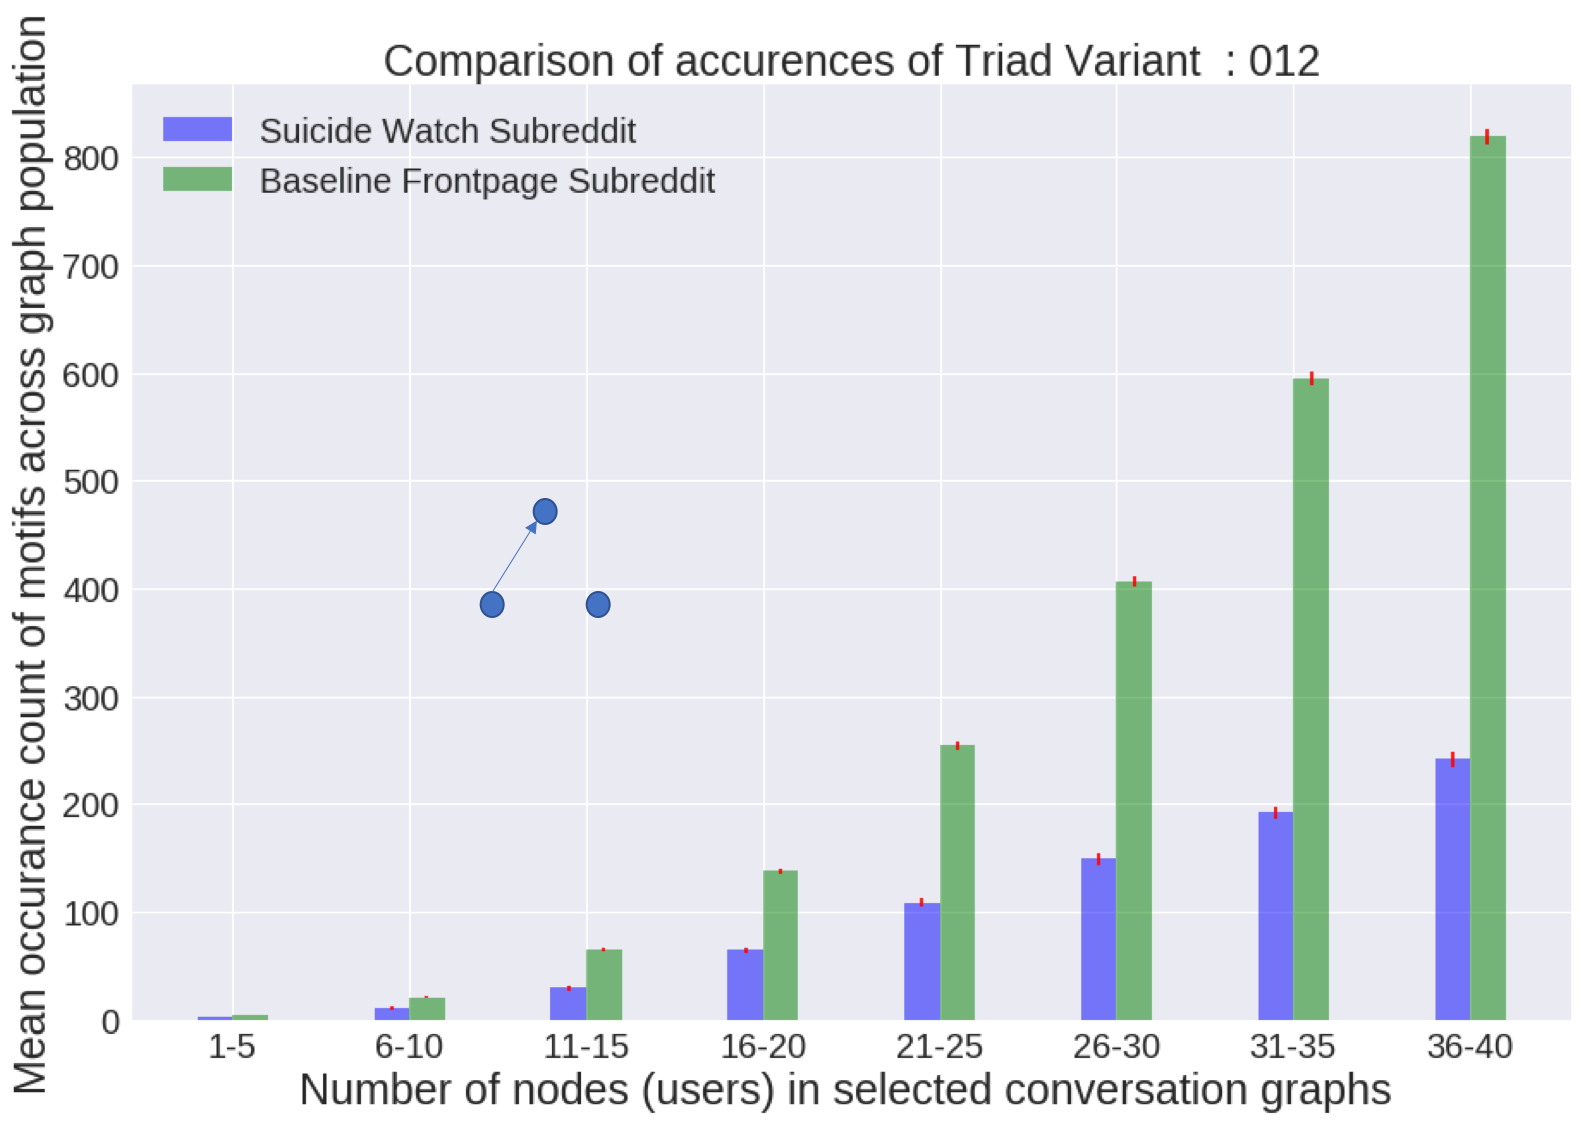
\includegraphics[width=0.5\linewidth ]{012.png}
        \label{fig:012_over}
    }
    \subfloat[]{
        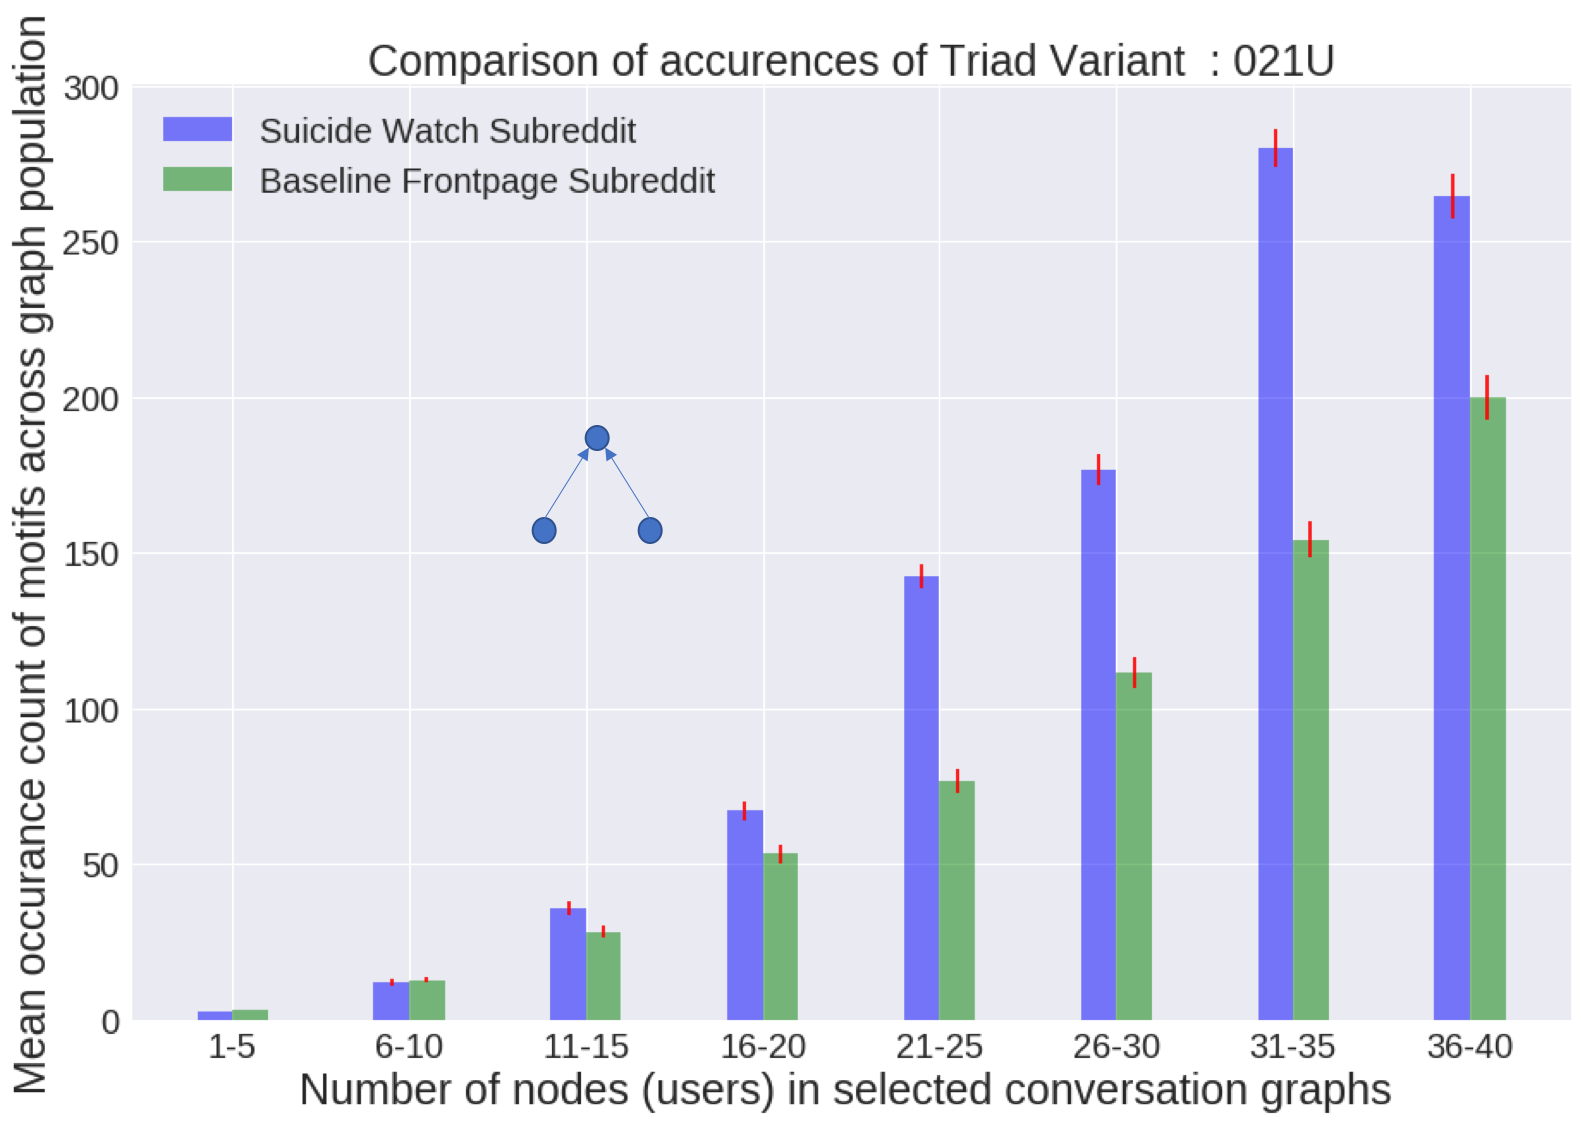
\includegraphics[width=0.5\linewidth ]{021U.png}
        \label{fig:021U_over}
    }
    
    %    \subfloat[]{
    %		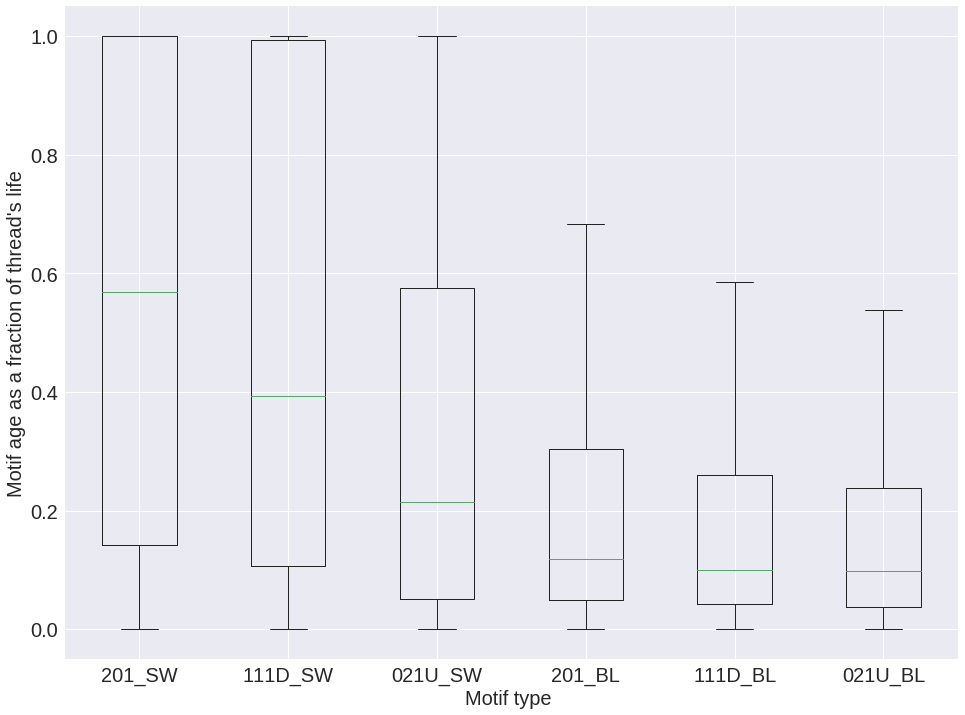
\includegraphics[width=0.5\textwidth, height = 6cm ]{Figures/BoxPlotMotifs_all.png}
    %		\label{fig:motifOccurance}
    %	}
    %	\subfloat[]{
    %		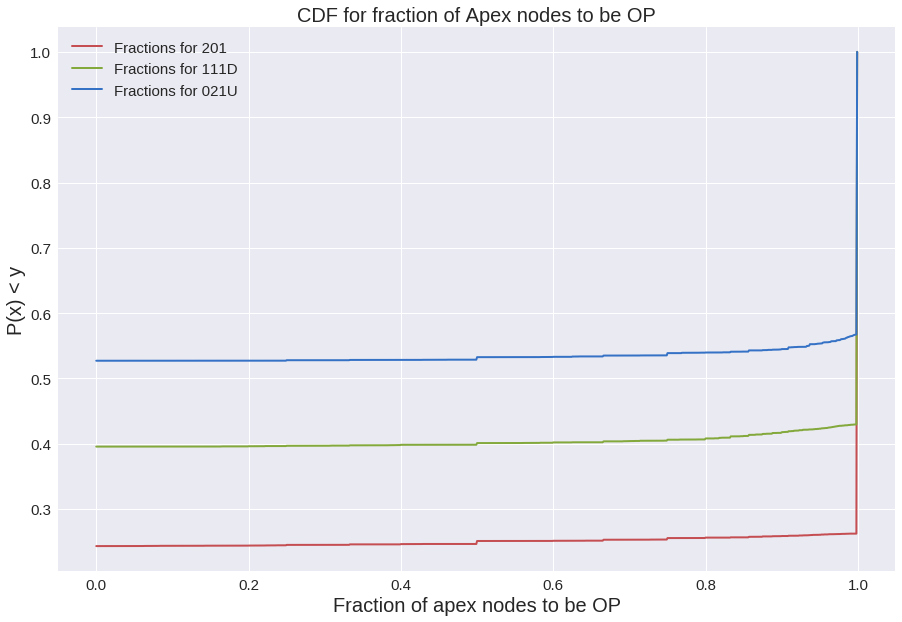
\includegraphics[width=0.5\linewidth, height = 6cm ]{Figures/CFD_ApexOP.png}
    %		\label{fig:ApexOPProp}
    %	}
    
    
    \caption{This panel shows the statistical significance of the three over expressed and one under expressed triadic motif. 
        %    Figure \ref{fig:motifOccurance} shows the distribution of each of the triadic motif's temporal point of occurrence according to the latest edge, as a proportion of the thread's lifetime. }
    }
    \label{Sec:motif}
\end{figure*}


\section{Methods}
This section discusses the methodological devices used to extract insights from the fora data.

\subsection{Data}
We build on dataset that was used in \cite{gkotsis2017characterisation} where they analyze textual content for the root posts in a Subreddit called Suicide Watch\footnote{\url{https://www.reddit.com/r/SuicideWatch/}}. The dataset contains a dump of 53 thousand posts from the suicide watch sub-reddit.
However the dataset did not contain the threaded conversations for each thread. Reddit is a platform where a user can create a post on a sub-reddit, to which several members of a given sub-reddit can interact with. The array of interactions may range from simple up or down votes or posting at different hierarchy of the thread. This creates a hierarchical threaded structure of posts where the conversations are organized as threads of posts. To understand the deeper structure that is present in these posts,  we crawl Reddit to get the threaded conversations by pursuing each conversation at arbitrary depth. \footnote{The code to crawl reddit for threads can be found at \textit{https://github.com/sagarjoglekar/redditTools}}. This results in a dataset of over 50 thousand threads totaling to around 500,000 individual posts on those threads.  

To baseline our work and compare theorized supportive nature of conversations with the broader community, we also crawl other reddit threads. To avoid any bias towards a particular type of subreddit, which have their own culture, we acquire roughly 50 thousand baseline posts which have been popular enough to land on the front page \footnote{The reddit front page algorithm is a combination of popularity and decay in popularity as a function of time. More can be found here \url{https://goo.gl/uVdHjn}}. We crawl the Frontpage posts for 2 weeks accumulating over 50 thousand reddit threads in the process. The median amount of responses for a Suicide watch thread were 6 and for baseline Frontpage posts were 8. 
To understand the structure of these two foras, and find discriminating factors between a supportive community like suicide watch and a general thread on Reddit, we need to build abstractions of the thread. 



%
%\subsection{Semantic similarity}
%\label{Topic}
%\sj{Change this, We are using word2vec now}
%To capture the content features of the reddit posts, we use Topic modeling\cite{Blei2003} to extract topic features from the corpus of posts. LDA converts a document $D$ into a $N$ dimensional vector of probabilities of $N$ topics , where the value of $N$ is selected using maximum variance method\cite{Sievert2014}. We train two LDA topic models one for the Suicide watch Corpus $F_{SW}$ and one for the Baseline corpus $F_{BL}$. The model $F_{SW}$ is trained on a corpus of 800,000 posts on the suicide watch sub-reddit and the model $F_{BL}$ is trained on a baseline of 1.5 million posts on the frontpage threads. These models are then later used to extract semantic information from post text T,  $F(T) \mapsto [t_0 , t_1 \ldots t_n ]$ where $t_k$ is the vector of topics that are present in text $T$


%\subsection{Networked conversations}
% \begin{table}
% 	\resizebox{0.5\linewidth}{!}{
% 		\begin{tabular}{l|p{8cm}}
% 			\textbf{Terminology} & \textbf{stands for}\\
% 			$RP$   & Root post which begins a new thread on a subreddit \\
% 			$OP$  & Original poster who posts the Root post for a thread \\
% 			$BP$   & A Poster who has at-least one symmetric response from the $OP$ after his comment\\
% 			$AP$   & Asymmetric poster who responds to $OP$ but never gets a response back \\
% 			$SW$ & The suicide watch Subreddit \\
% 			$FP$  & Front page of Reddit. \\
% 	\end{tabular}}
% 	\caption{Notations and Terms.}\label{notations}
% \end{table}


\subsection{Abstractions}
\label{Sec:Abstractions}
To understand the dynamics of supportive conversations, we first need to formalize the abstraction of networked conversations. In case of forum based platforms where users interact in a nested dialogue fashion, and original poster or $OP$ posts a start of a thread. This thread is then open for comments by all the community users. In case of Reddit, such a community is called a Subreddit, which is a moderated collection of users who subscribe to it. These users may post new threads onto the subreddit as far as the post follows the subreddit rules. Enforcement of these rules is the responsibility of the moderators. The user who starts a thread is called the Original Poster or \textbf{OP} and the headlining post which the $OP$ begins with is called the Root Post or $RP$. 


\label{Sec:network}

\begin{figure*}[!ht]
    \centering
    % \hspace*{-5mm}
    \subfloat[]{
        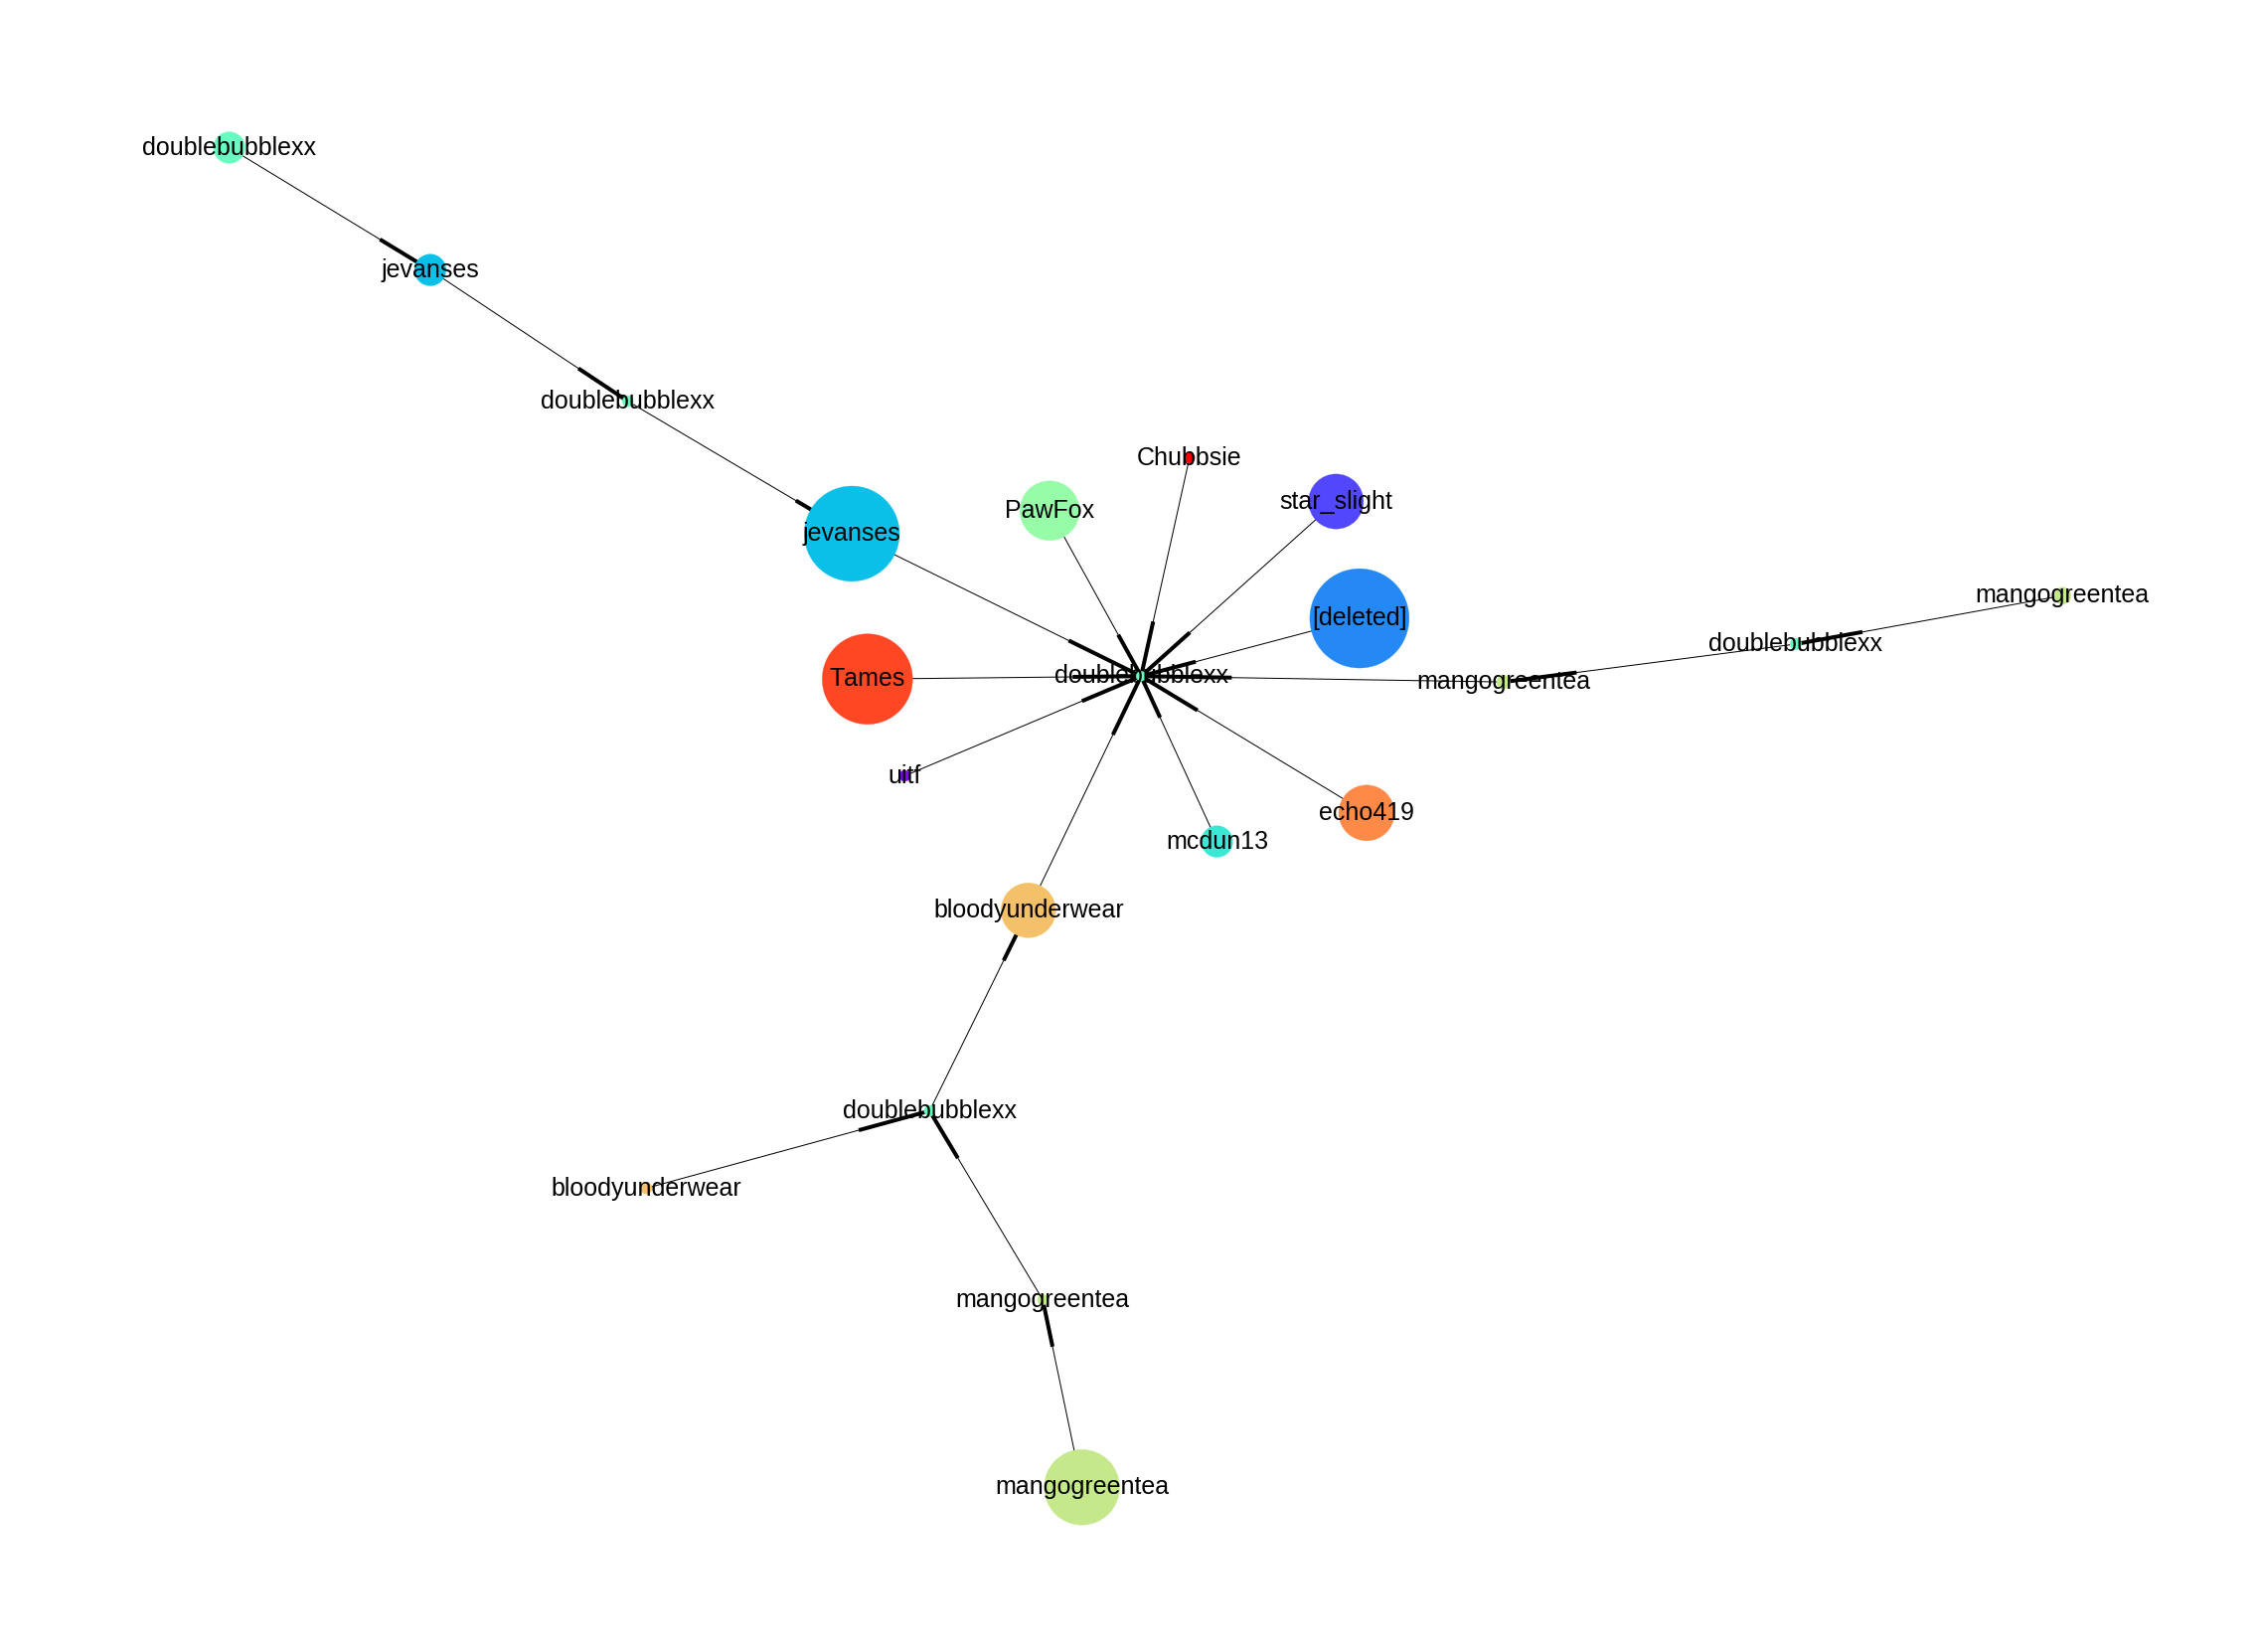
\includegraphics[width=0.45\textwidth, height = 5cm ]{ReplyGraphSW}
        \label{fig:rGraphSW}
    }
    \subfloat[]{
        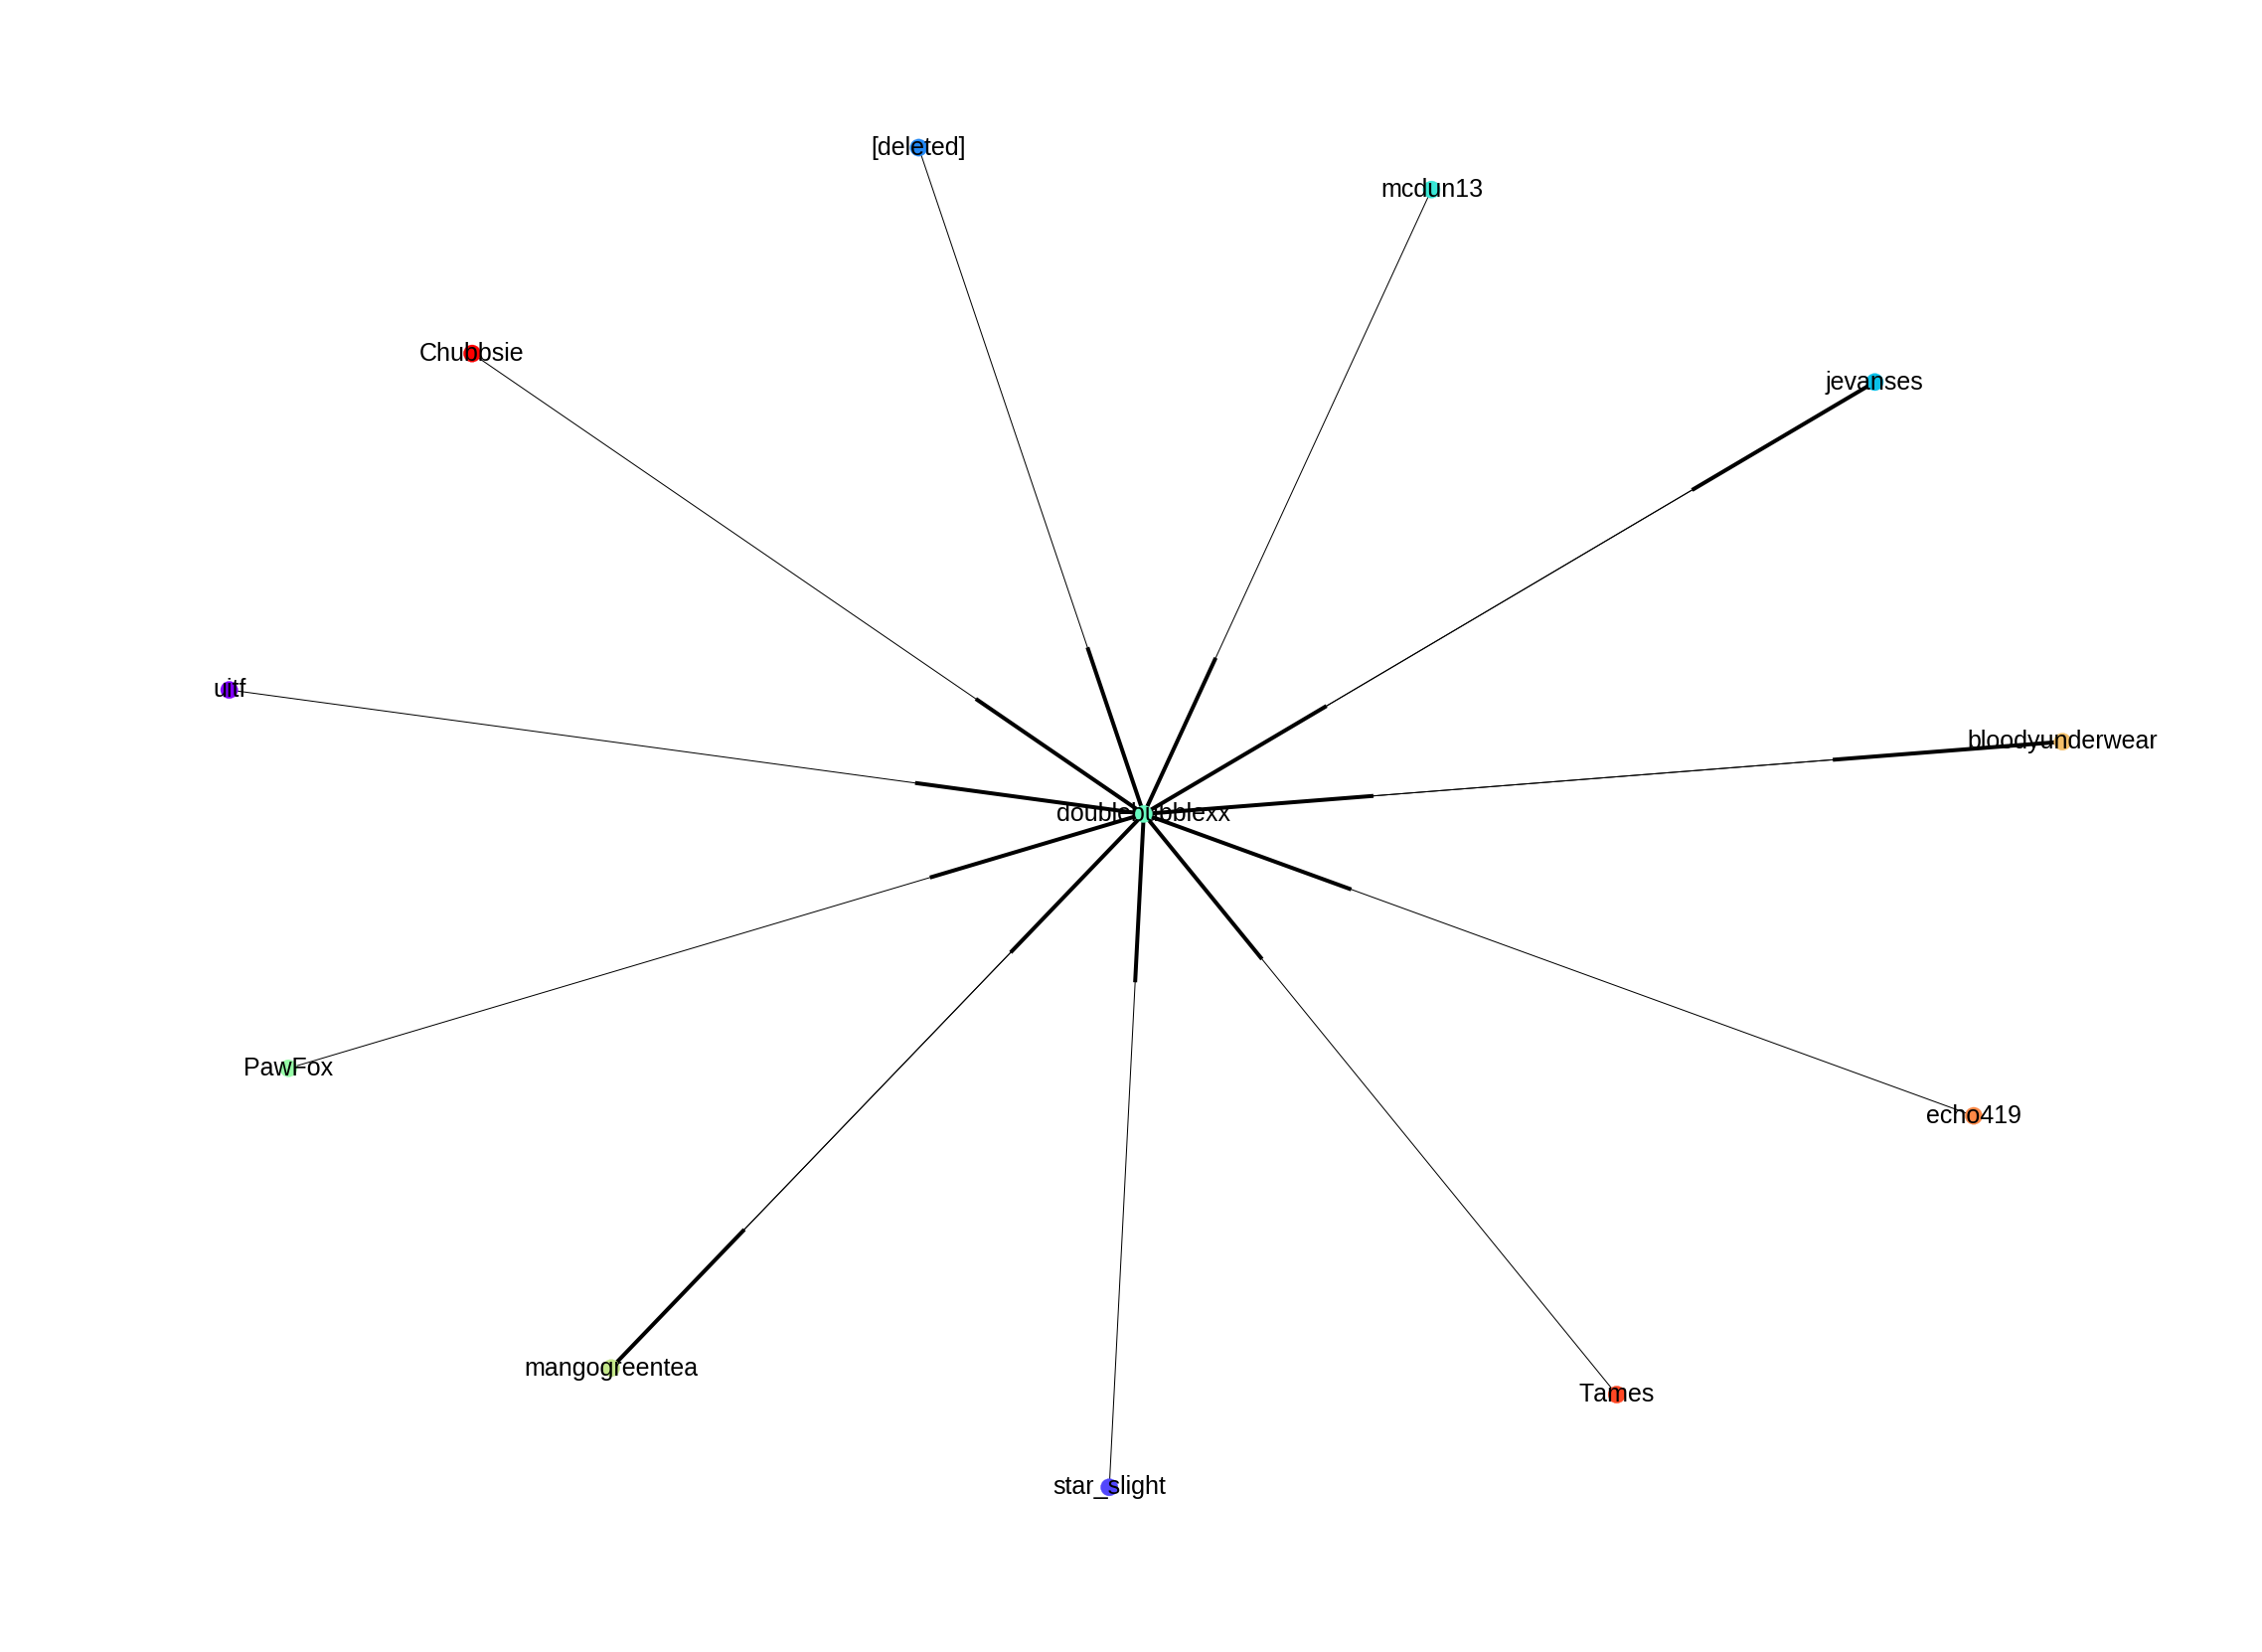
\includegraphics[width=0.45\linewidth, height = 5cm ]{UserGraphSW}
        \label{fig:uGraphSW}
    }
    
    
    \subfloat[]{
        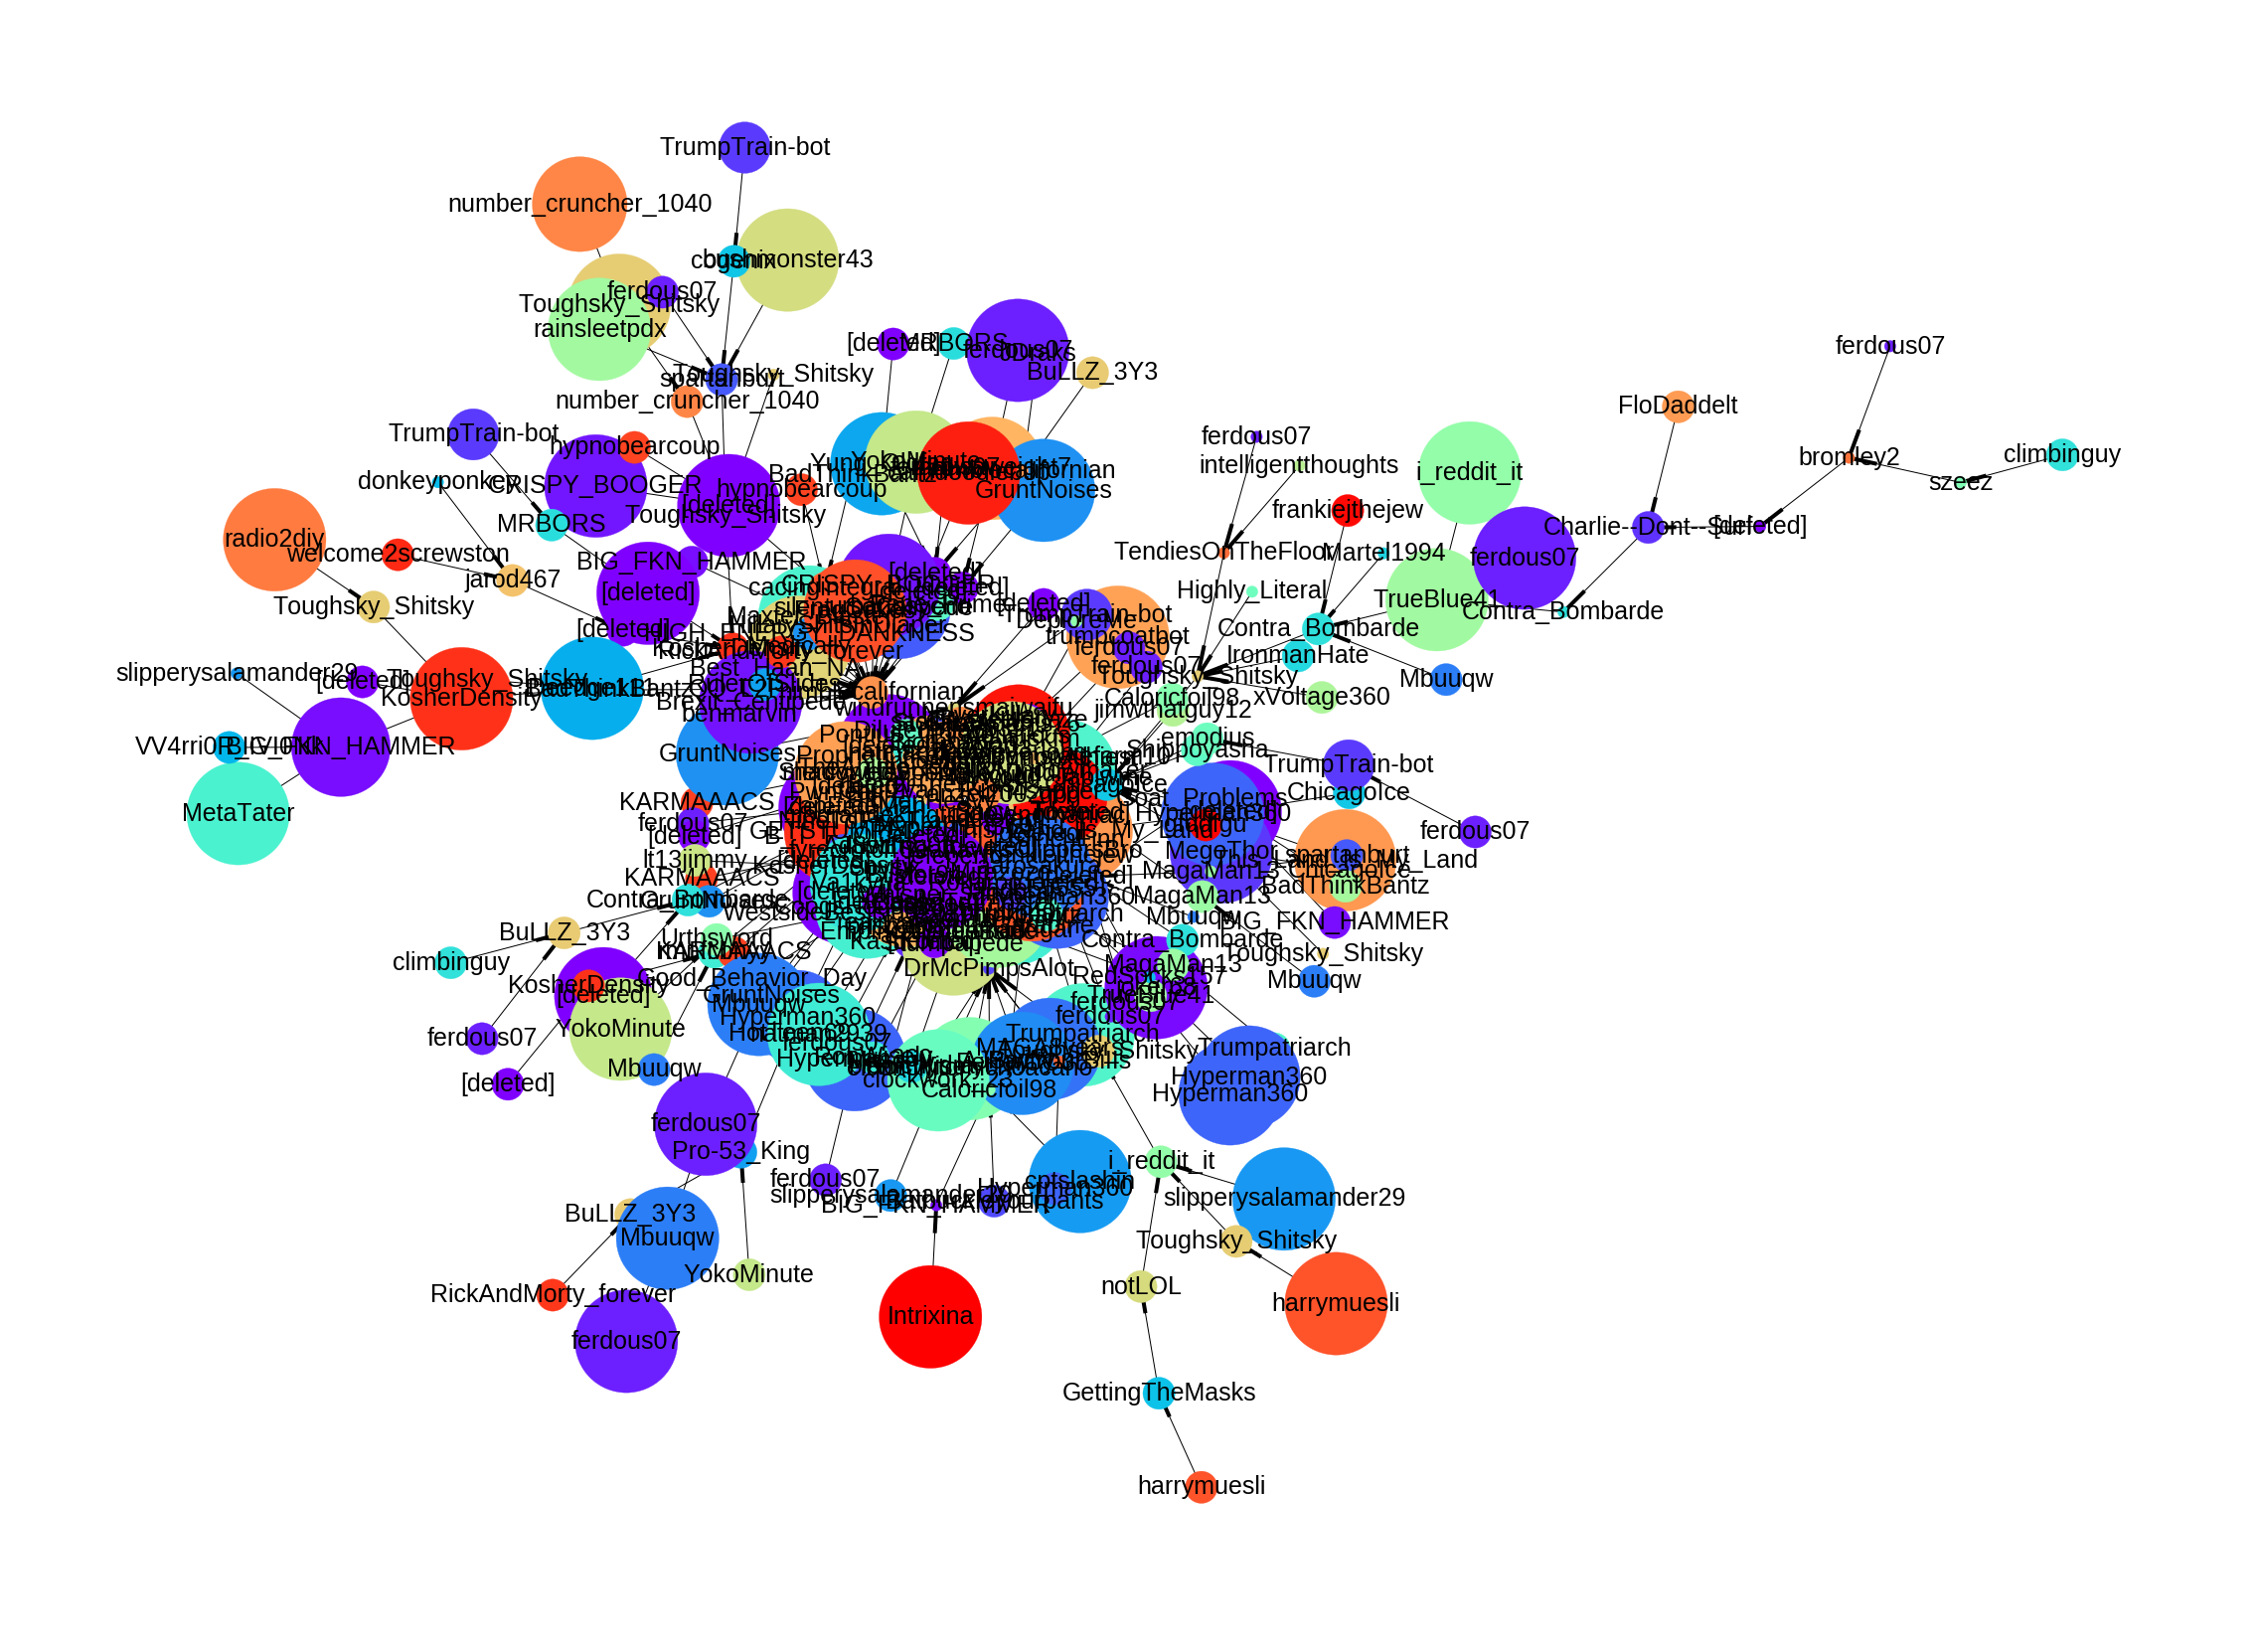
\includegraphics[width=0.45\linewidth, height = 5cm ]{ReplyGraphTD}
        \label{fig:rGraphTD}
    }
    \subfloat[]{
        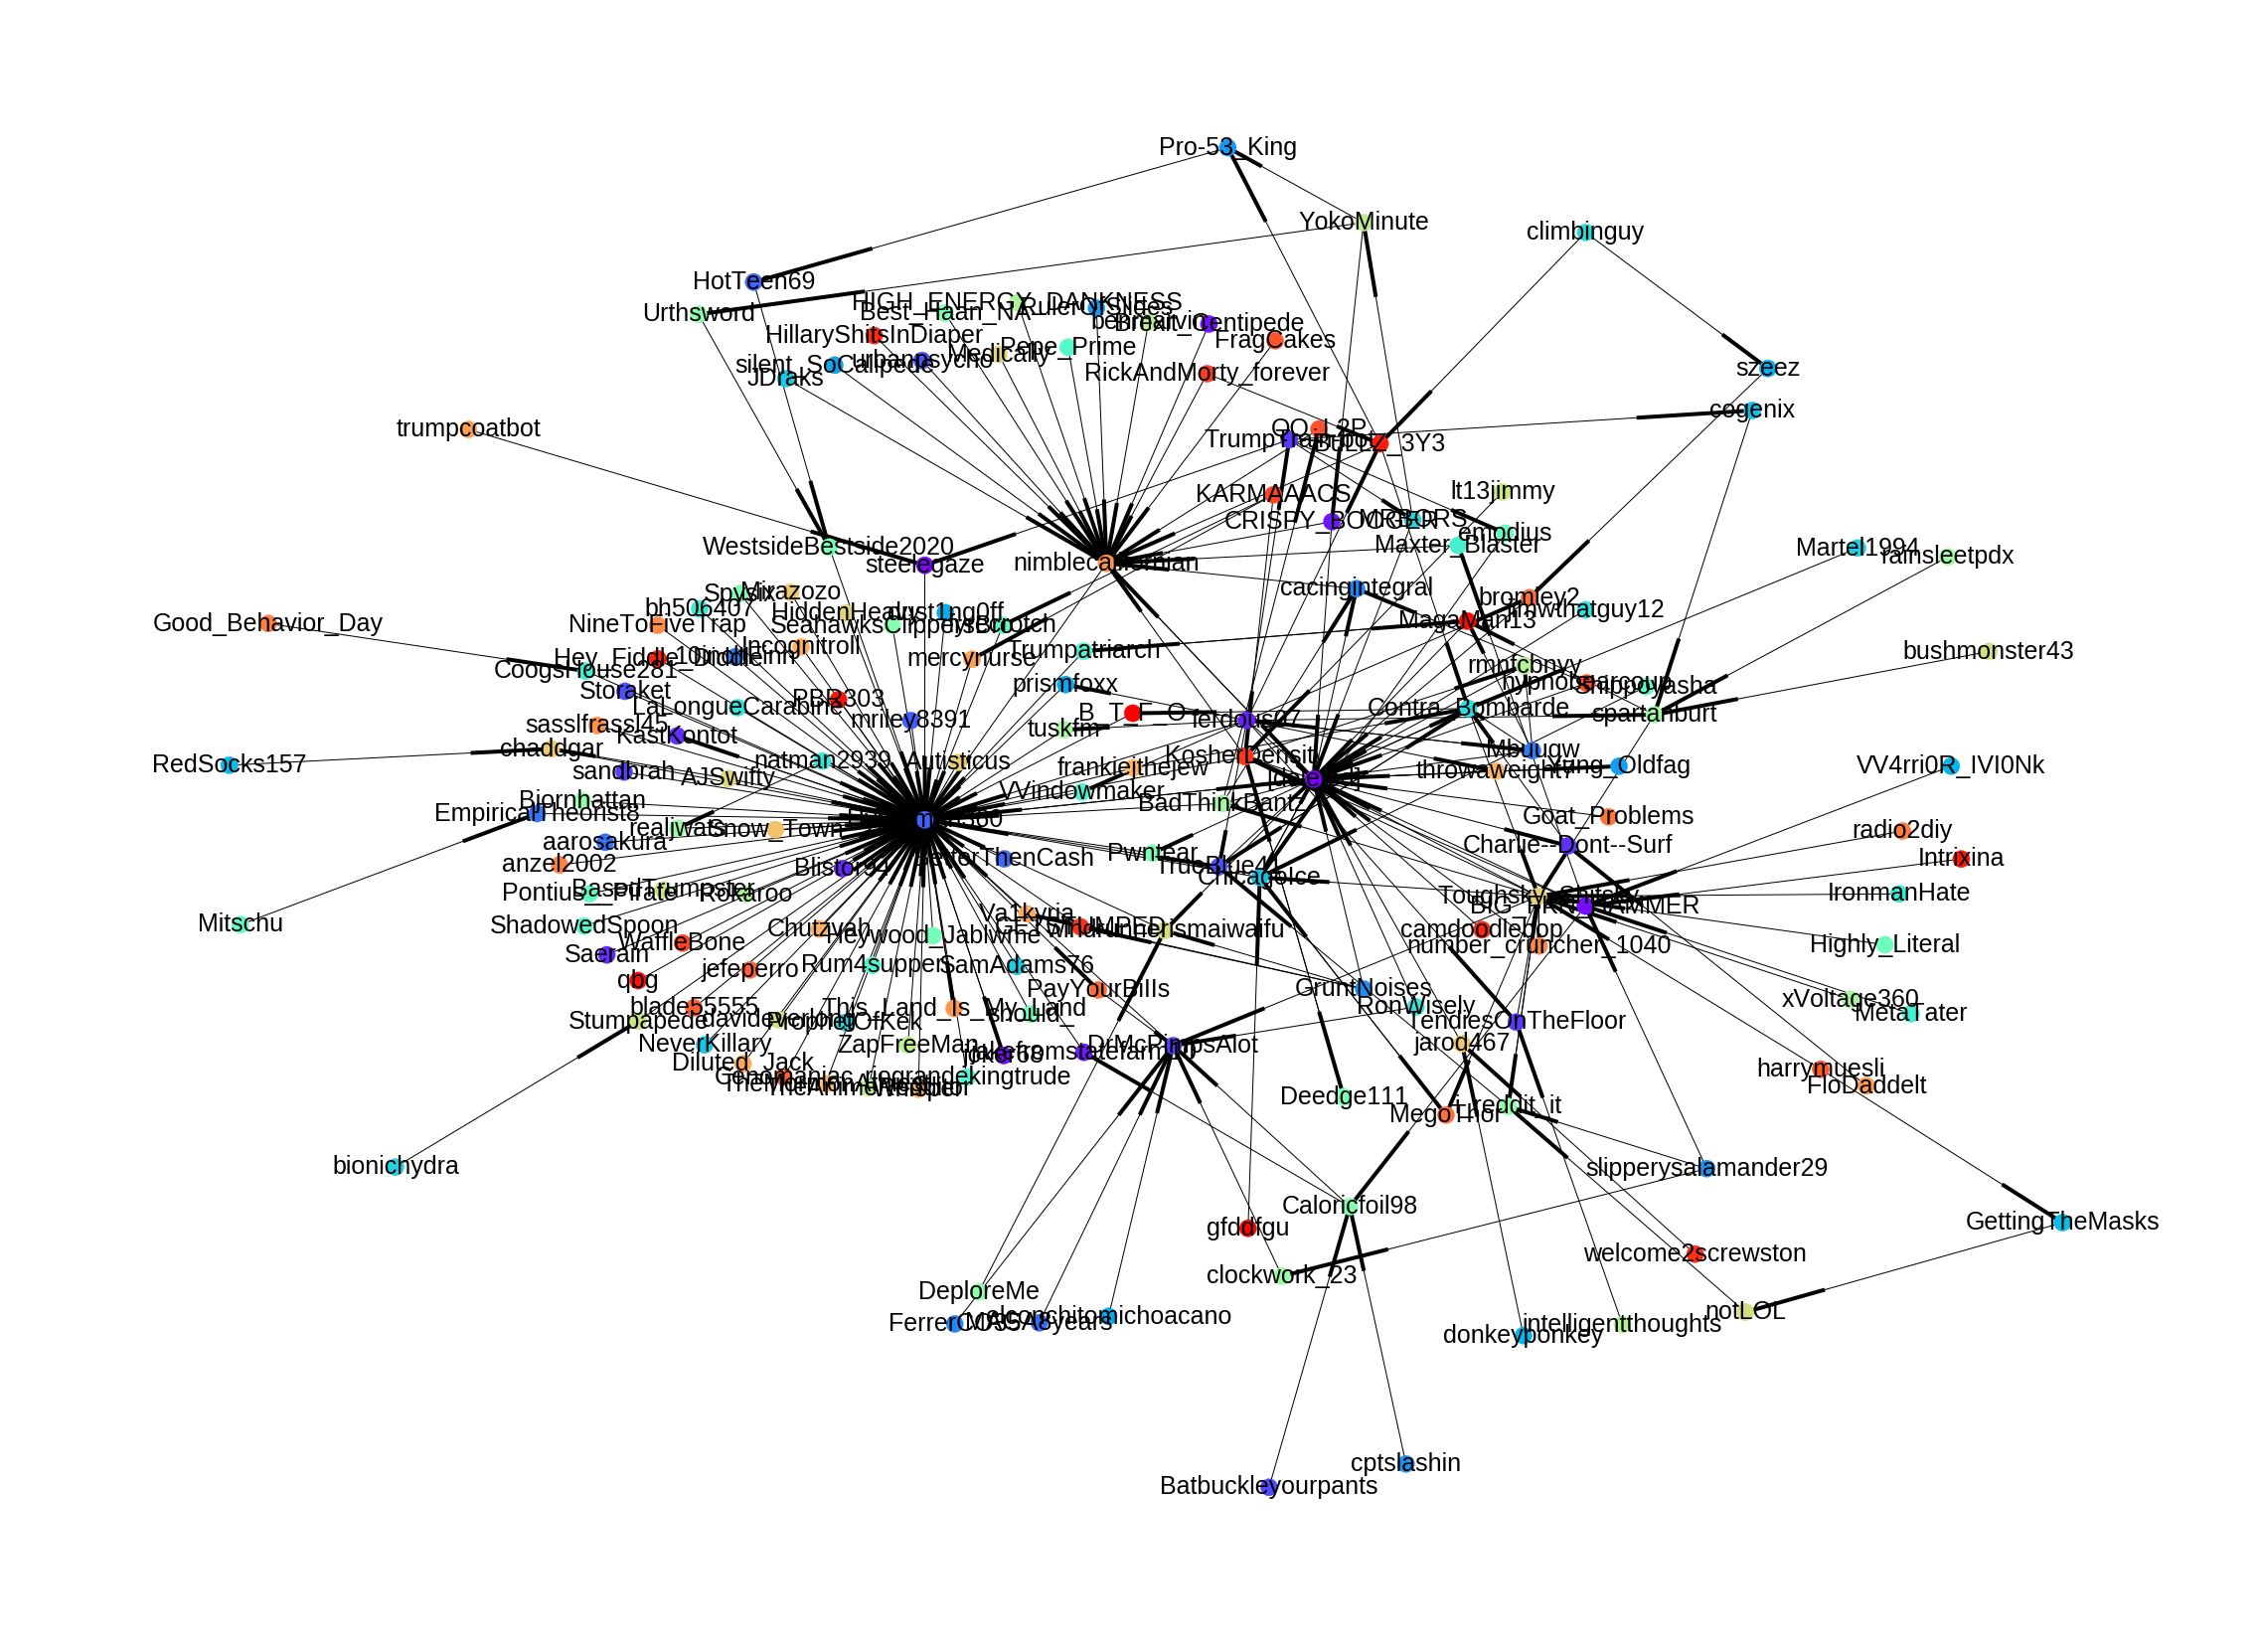
\includegraphics[width=0.45\linewidth, height = 5cm ]{UserGraphTD}
        \label{fig:uGraphTD}
    }
    \caption{ Example UserGraphs and their corresponding Reply graphs, Figure \ref{fig:uGraphSW} shows a random thread from the SW sub-reddit and \ref{fig:rGraphSW} shows the corresponding reply graph that arises from the response structure of the same thread. In comparison we have Usergraph Fig \ref{fig:uGraphTD} and its corresponding reply graph Fig \ref{fig:rGraphTD} from one of the Front page threads }
    \label{Fig:GraphExamples}
\end{figure*}



\subsubsection{Reply Graphs}
\label{Sec:Reply_graphs}
The first abstraction mimics directly the structure of conversation threads on Reddit. These abstractions are called Reply Graphs. We formulate a reply graph $R\{P,E,W\}$ as a thread of multi-layered posts in a thread in response to the root post $RP$ in the sub-reddit. Each graph $R$ consists of posts $P_i , P_j , i,j \in N$ , where N+1 is the total number of responses in the thread and Edges $E_{ij}$such that and Edge $E_{ij}$ exists $iff$ post $P_i$ was in response to post $P_j$ in the hierarchy of responses.  The weight of the edge $E_{ij}$ is found by calculating the cosine similarity between topic vector $T_i$ for post $P_i$ and the topic vector $T_j$ of post $P_j$. For a given dataset, the topic vectors are extracted using the model trained on that particular corpus ($LDA_{BL}$, $LDA_{SW}$).  This abstraction works well in modeling the conversational nature of these forums.  For convenience of the reader, we present a couple of example pairs from SW and Frontpage baseline datasets in Figure \ref{Fig:GraphExamples}

\subsubsection{Interaction Graphs}
\label{Sec:Interaction_graphs}
In this method, we represent each thread as a directed graph $G\{V,E,W\}$ where $V$ is the set of all users participating in a particular thread and $E$ are the directed  edges which correspond to interactions between two users $V_i , V_j  \in V$. The weight of each directed edge $E_{ij}$ corresponds to the average of all the edges between $V_i , V_j  \in V$ in the corresponding reply graph $R\{P,E,W\}$ as described above. This means that each reply graph is then mapped to a User graphs where the nodes are Users rather than posts. Another salient distinction between the two abstractions is that reply graphs resemble an n-ary tree and user graphs are directed cyclic graphs. 





\subsection{Macro and local metrics}
The abstractions are used to extract certain structural metrics from the conversation threads. These metrics are then used to validate structural differences between supportive conversations and generic casual conversations from out baseline set.


\subsubsection{Centrality}
\label{Sec:Centrality}
For this metric we use the User Graphs. Node centrality is a metric that measures how central a node is in a network. It directly reflects the importance of the node when it comes to membership of the shortest connecting paths between all the nodes in the graph. More formally, we use betweenness centrality of a node which is defined as 
Betweenness centrality of a node $v$ is defined as 
$$
g(v) = \sum_{s \neq v \neq t}\frac{\sigma_{st}(v)}{\sigma_{st}}
$$
where $\sigma_{st}(v)$ is the total number of shortest paths from node $s$ to node $t$ and $\sigma_{st}$ is the number of those paths that pass through $v$. To understand whether the thread starters ($OP$) have a special place in the network, we evaluate both $OP$ centrality as well as median centrality across all the nodes in a User graph.

\subsubsection{Symmetrical users}
We define a symmetric user and a symmetric edges for user graphs. For a user $V_i$ in the user graph $G\{V,E,W\}$ as described in Section
, a symmetric user is a user who interacts with $V_o$ or the $OP$ and receives a response back from the $OP$. We find the fraction 
$$
U_{sym}=\frac{\textit{total number of symmetric users }}{\textit{Total users in a thread}}
$$

\subsubsection{Urgency}
To understand how Suicide watch subreddit users responds to the $OP$ and each other, compared to other sub-reddit threads on the frontpage, we calculate differences between the posting times between consecutive messages in a reply graph. We compute the median response times per thread, for $OP$'s posts and for all other posts. 

\subsubsection{Branching Factor}
\label{Sec:Branching}
Branching factor is a quantity that reflects the fan out of a conversation as it evolves.
To measure this phenomena, we use the reply graphs, which resemble a n-ary directed acyclic graph, to evaluate the branching factor. The branching factor is formally described as 
$$\tau = \frac{1}{|D|} \sum_{d \in D}^{} \frac{1}{|N_d|} \sum_{n\in N_d}^{} \textit{InDeg}(n)$$


\subsubsection{Response distance}
A user who interacts frequently with a thread, may contribute at different stages of hierarchy. Intuitively, for a one on one conversation to exist, the user needs to contribute back to the thread at alternate levels of hierarchy. To measure this phenomenon, we assume that a user $U$ contributes in a reply graph at variable depths $d_i \forall i \in [0,D]$. 
We calculate the average difference between two consecutive contributions $d_{avg}$
$$ d_{avg} = \frac{\sum_{i=0}^{D} d_{i+1} - d_i }{D}$$
We calculate the values of $d_{avg}$ for both $OP$ and other users in the thread.


\subsubsection{Semantic similarity}
\label{Sec:Semantic}
We use a popular word embedding method called \textit{Word2Vec} \cite{mikolov2013distributed} which learns representations of a set of words from a corpus of text, which in our case is the text from Suicide Watch and baseline fora. These representations can be used to extract text embedding vectors for each post which belong to a $N$ dimensional space $R^N$. These vectors are tested for their alignment using cosine distance in $R^N$, which corresponds to semantic similarity in the textual space. This method is quite popular and used in community based question answering\cite{mihaylov2016semanticz}, Medical semantic similarity \cite{de2014medical} and other medical informatics applications\cite{zhu2017semantic}.



\subsection{Structural metrics}
\label{Sec:motif}
Network motifs are local sub-networks between 2 or 3 nodes. Such local patterns are highly useful in quantifying local interactions and the resulting macro structure of the network\cite{milo2002network}. They gave been used in a variety of applications and networks, from economics \cite{zhang2014dynamic} to cellular protein-protein interaction networks \cite{yeger2004network}. Hence we calculate census of 16 distinct \textsl{triadic motif} i.e. possible subgraphs that could be formed between any three chosen nodes. 

\note{This probably needs to be briefly introduced/explained earlier in the manuscript?}
To understand relation of local structures in interaction networks within a conversation with its , we compare the quantity called \textsl{motif occurrence ratio}. 
After calculating motif census across the dataset\cite{Batagelj2001}, we select progressive subsets of graphs from both datasets with nodes $n \in [k , k+4]$ $\forall$  $k \in \{1, 6 , 11 , 16 , 21 , 26 , 31 , 36\}$. This segmentation of the dataset is called binning, and it allows us to not only measure the differences in the census between the datasets, but also observe the trend as the size of the interaction graph becomes larger. We stop at 40 because beyond that, we start getting lower and lower number of graphs samples per bin.  

We test each graph for the frequency of occurrence of the 16 possible triadic motifs as shown in Figure\ref{fig:motifs}. We start by selecting the subset of graphs from Suicide watch and Frontpage belonging to a particular bin $k$. 
%Lets call these sets of graphs $\K_{SW}$ and $\K_{BL}$ respectively. 
%Let us assume that for a given value of $k$ , $\Kappa_{SW}$ has $K_{SW}$ graphs and $\Kappa_{BL}$ has $K_{BL}$ graphs. We then count for a given motif, number of occurrences in $\Kappa_{SW}$ and $\Kappa_{BL}$ where the graph had at-least one instance of that motif. Let us call the total number of gra phs in $\Gamma_{BL}$ with a given motif as $\gamma_{BL}$ and $\gamma_{SW}$ likewise for the $\Gamma_{SW}$ graphs. 
We then define the motif occurrence ratio as the fraction values for $\frac{\gamma_{BL}}{K_{BL}}$ and $\frac{\gamma_{SW}}{K_{SW}}$ for all the 16 motifs across all the chosen values of $n$. 


\begin{figure*}[!h]
    \centering
    % \hspace*{-5mm}
    \subfloat[]{
        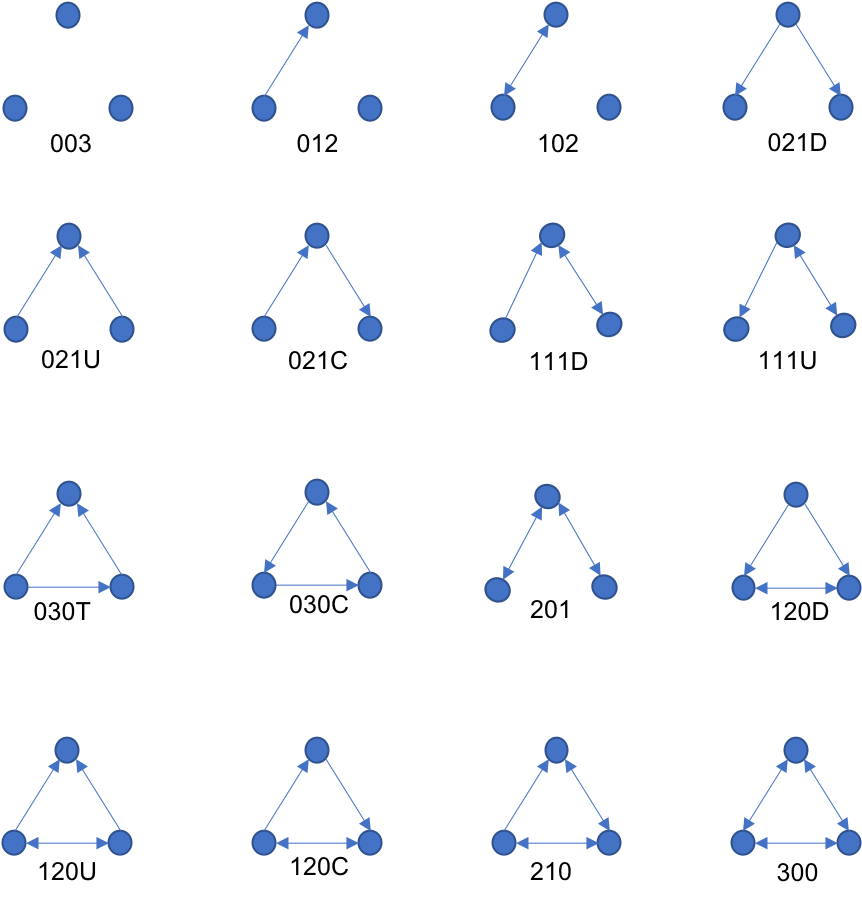
\includegraphics[width=0.7\textwidth]{TriadVariants}
        \label{fig:motifs}
    }
    
    \subfloat[]{
        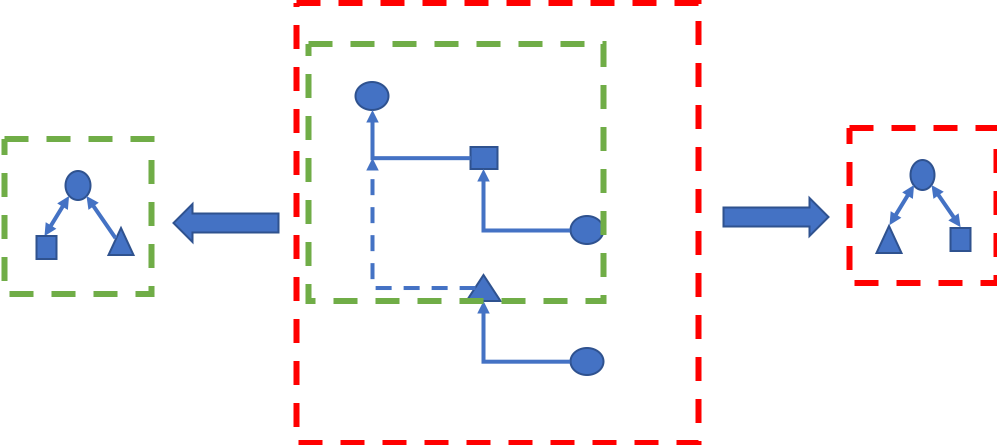
\includegraphics[width=0.7\linewidth, height = 5cm ]{thread}
        \label{fig:motifStruct}
    }
    \caption{ Figure \ref{fig:motifs} shows the 16 different types of motifs that are looked for in the user graph data. Figure \ref{fig:motifStruct} shows how three unique users could produce different motifs. The three shapes represent different users and the dotted line means the message order is irrelevant.}
    \label{Fig:motifs}
\end{figure*}




\section{Appendix}

\subsection{Triadic statistics for twitter conversations}

\begin{figure*}[!h]
    \centering
    % \hspace*{-5mm}
    \subfloat[]{
        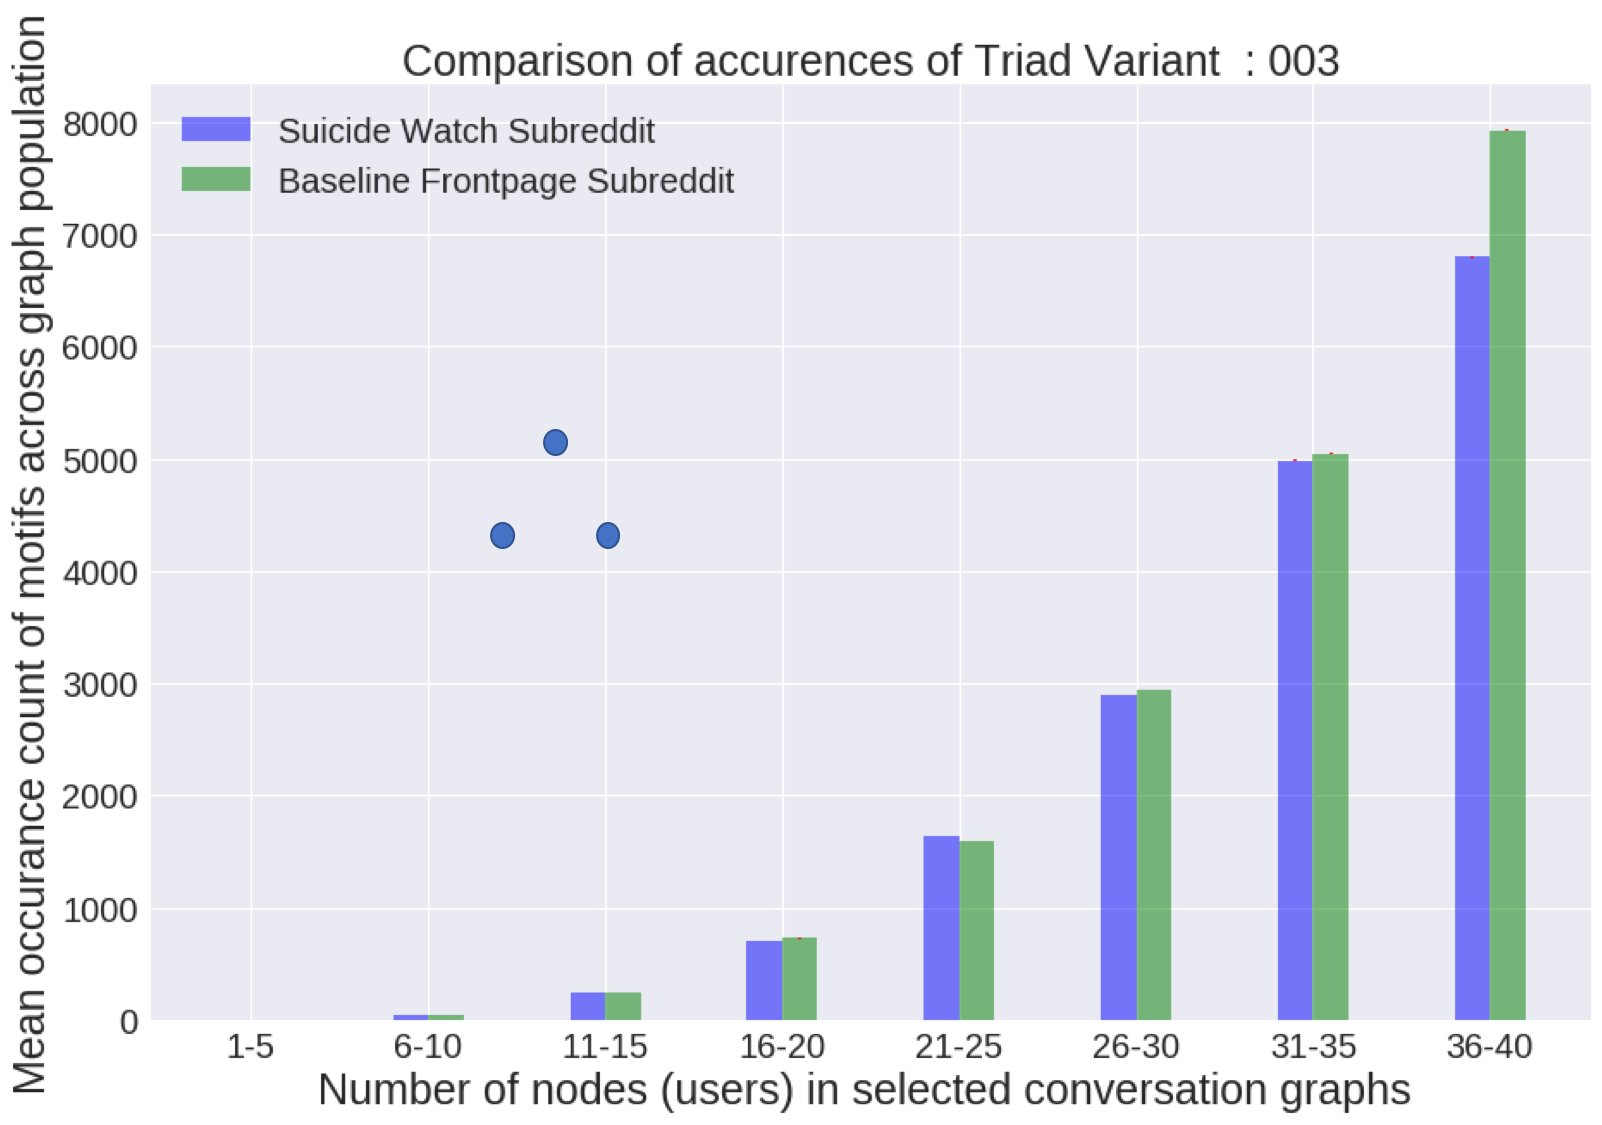
\includegraphics[width=0.33\textwidth, height = 4.5cm ]{003}
        \label{fig:003}
    }
    \subfloat[]{
        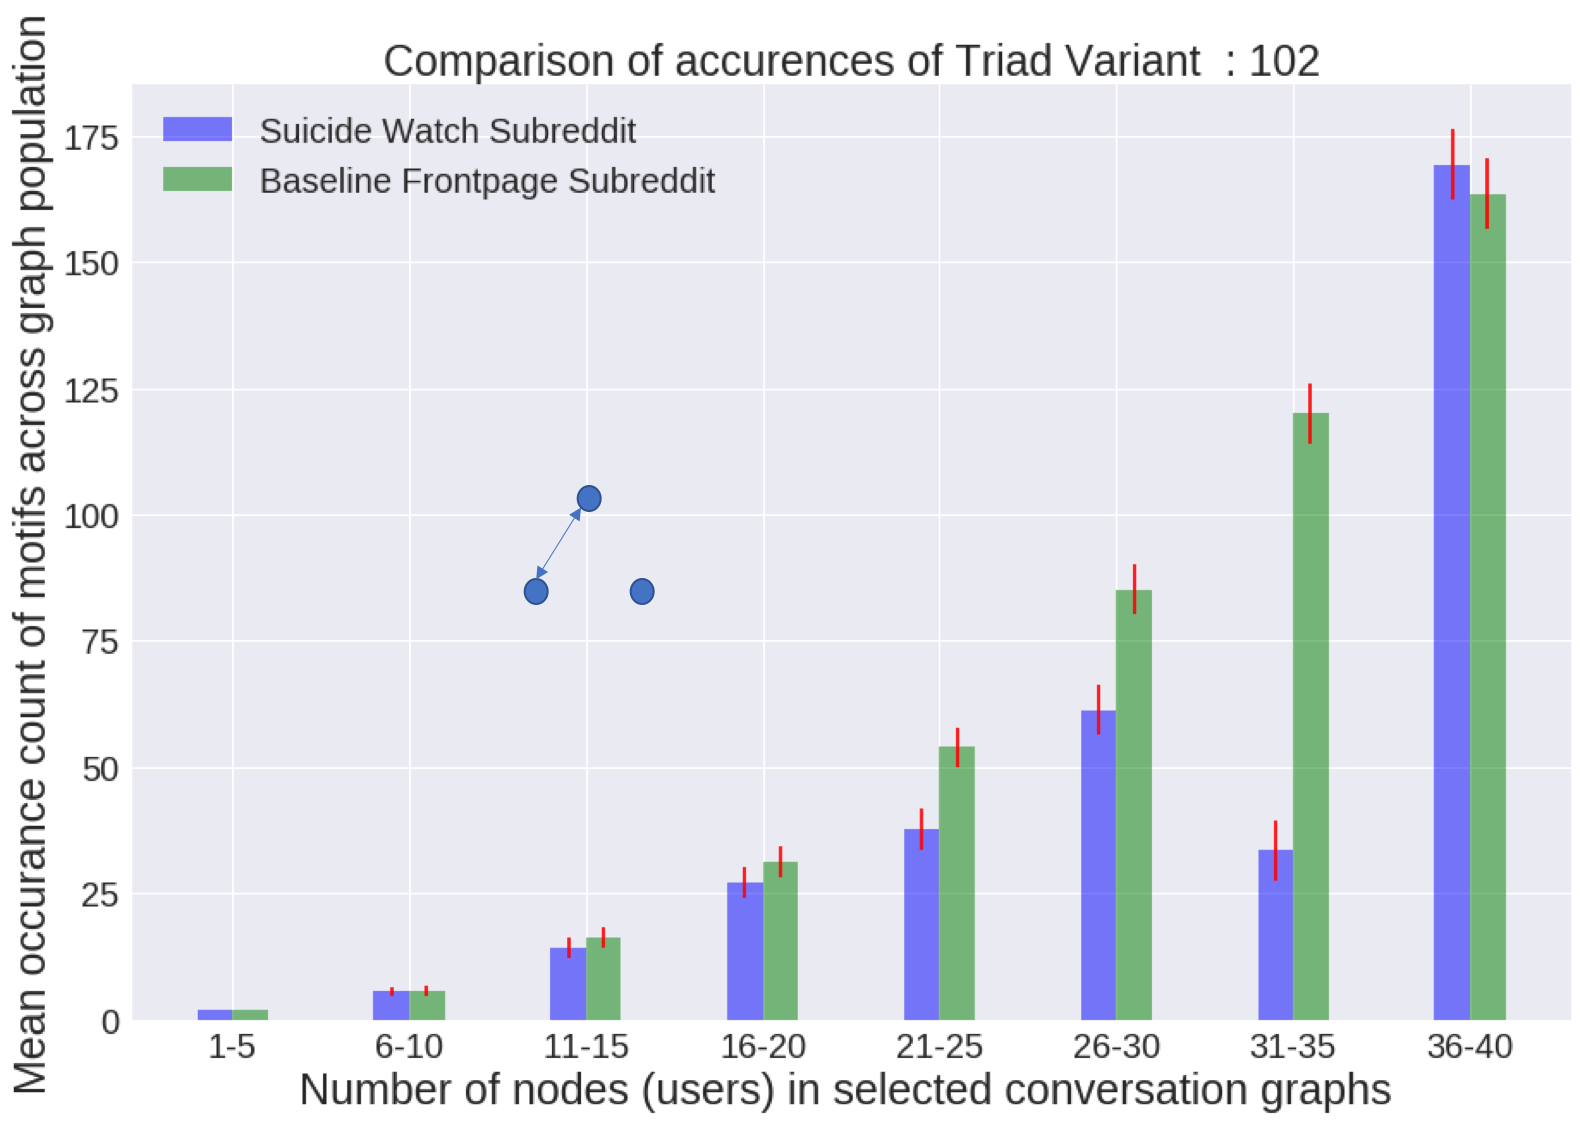
\includegraphics[width=0.33\textwidth, height = 4.5cm ]{102}
        \label{fig:102}
    }
    \subfloat[]{
        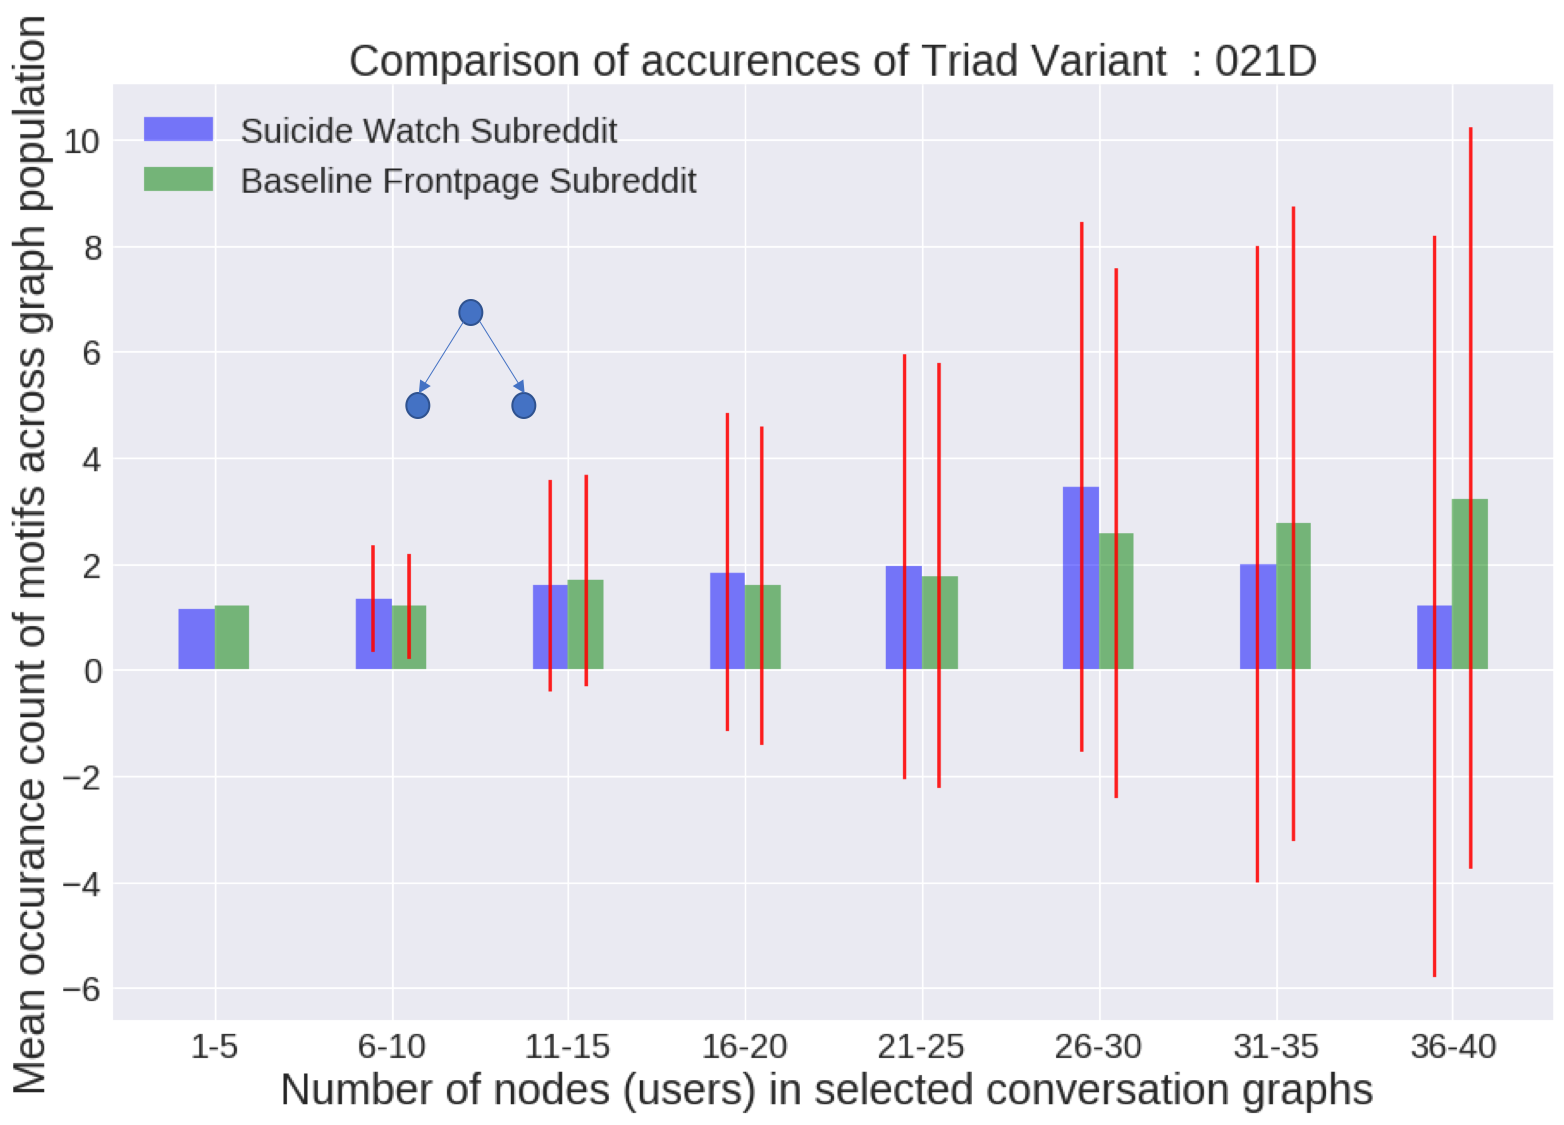
\includegraphics[width=0.33\textwidth, height = 4.5cm ]{021D}
        \label{fig:021D}
    }
    
    
    \subfloat[]{
        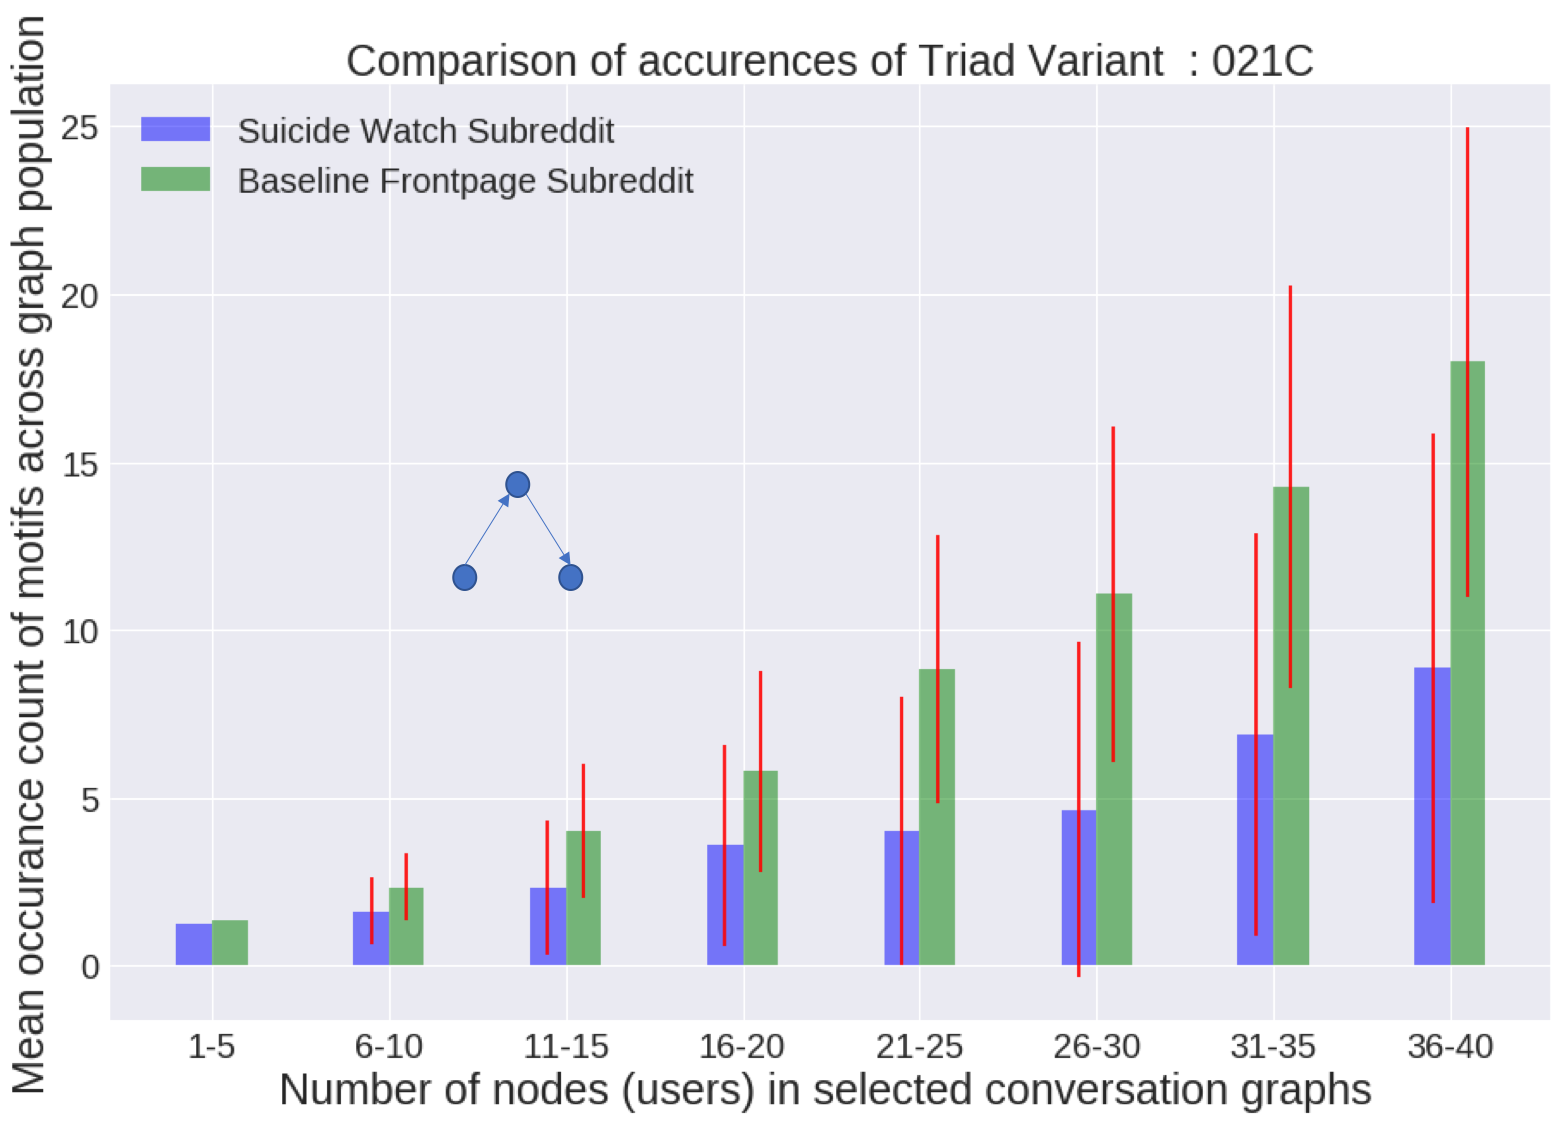
\includegraphics[width=0.33\textwidth, height = 4.5cm ]{021C}
        \label{fig:021C}
    }
    \subfloat[]{
        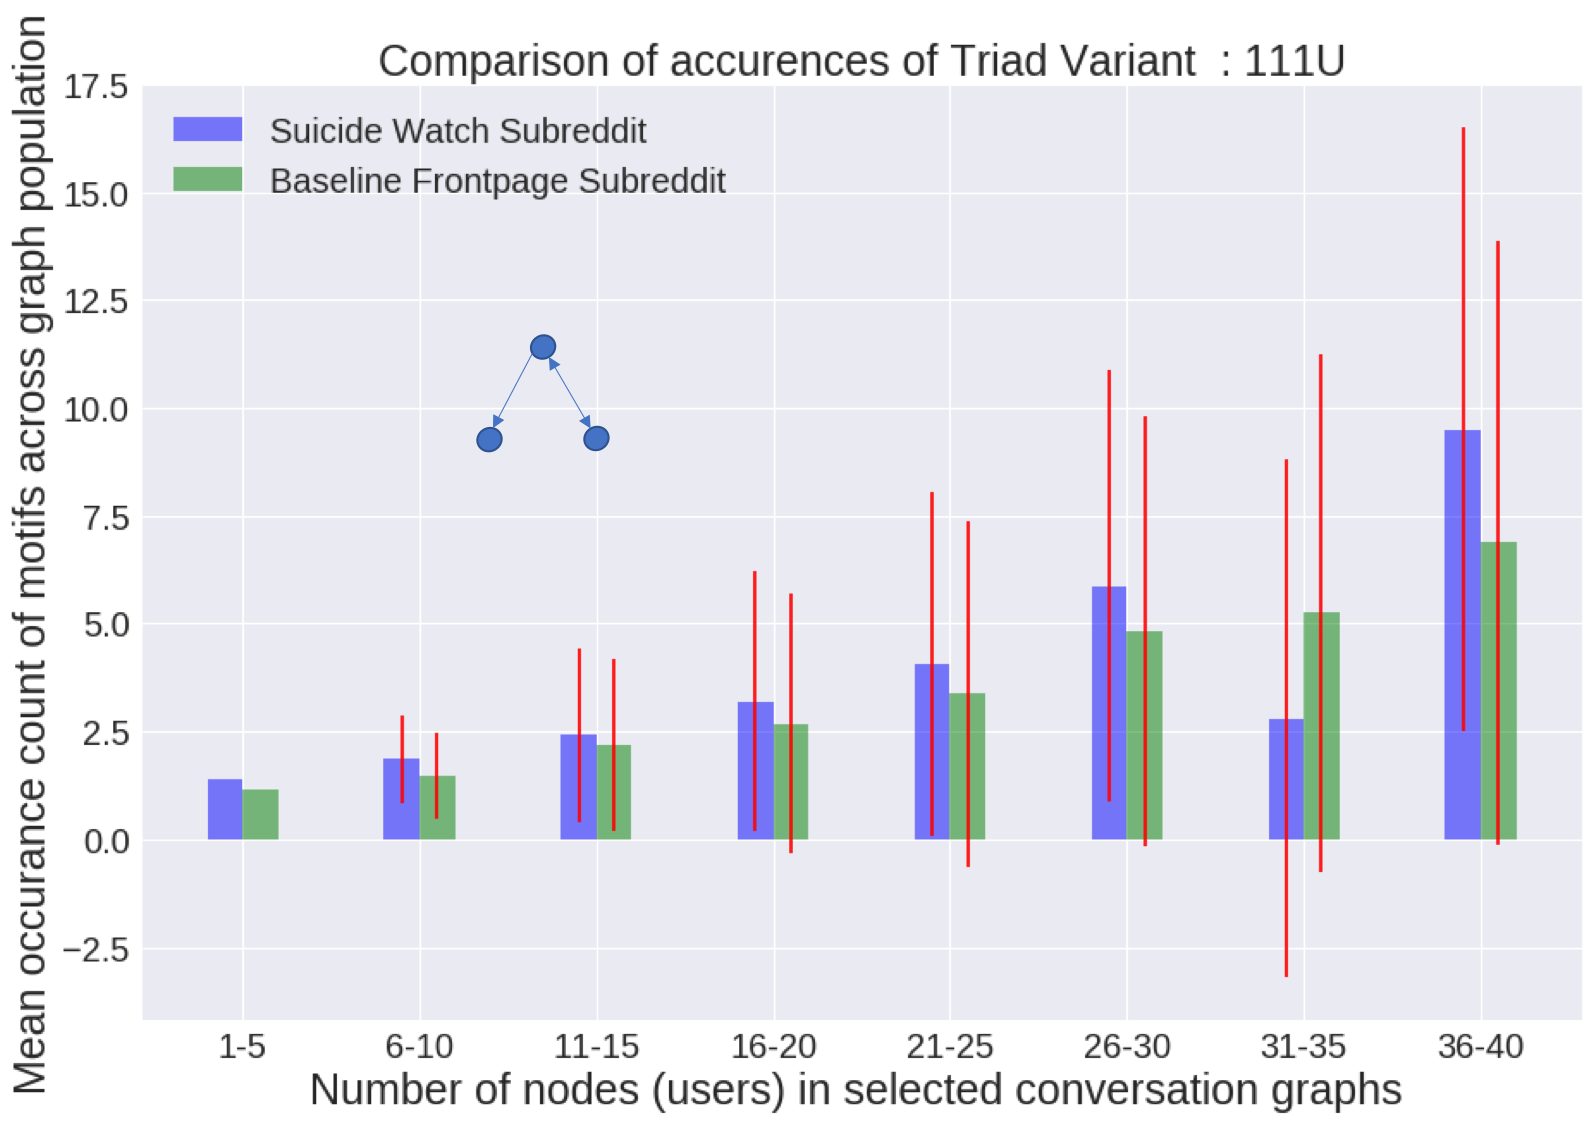
\includegraphics[width=0.33\textwidth, height = 4.5cm ]{111U}
        \label{fig:111U}
    }
    \subfloat[]{
        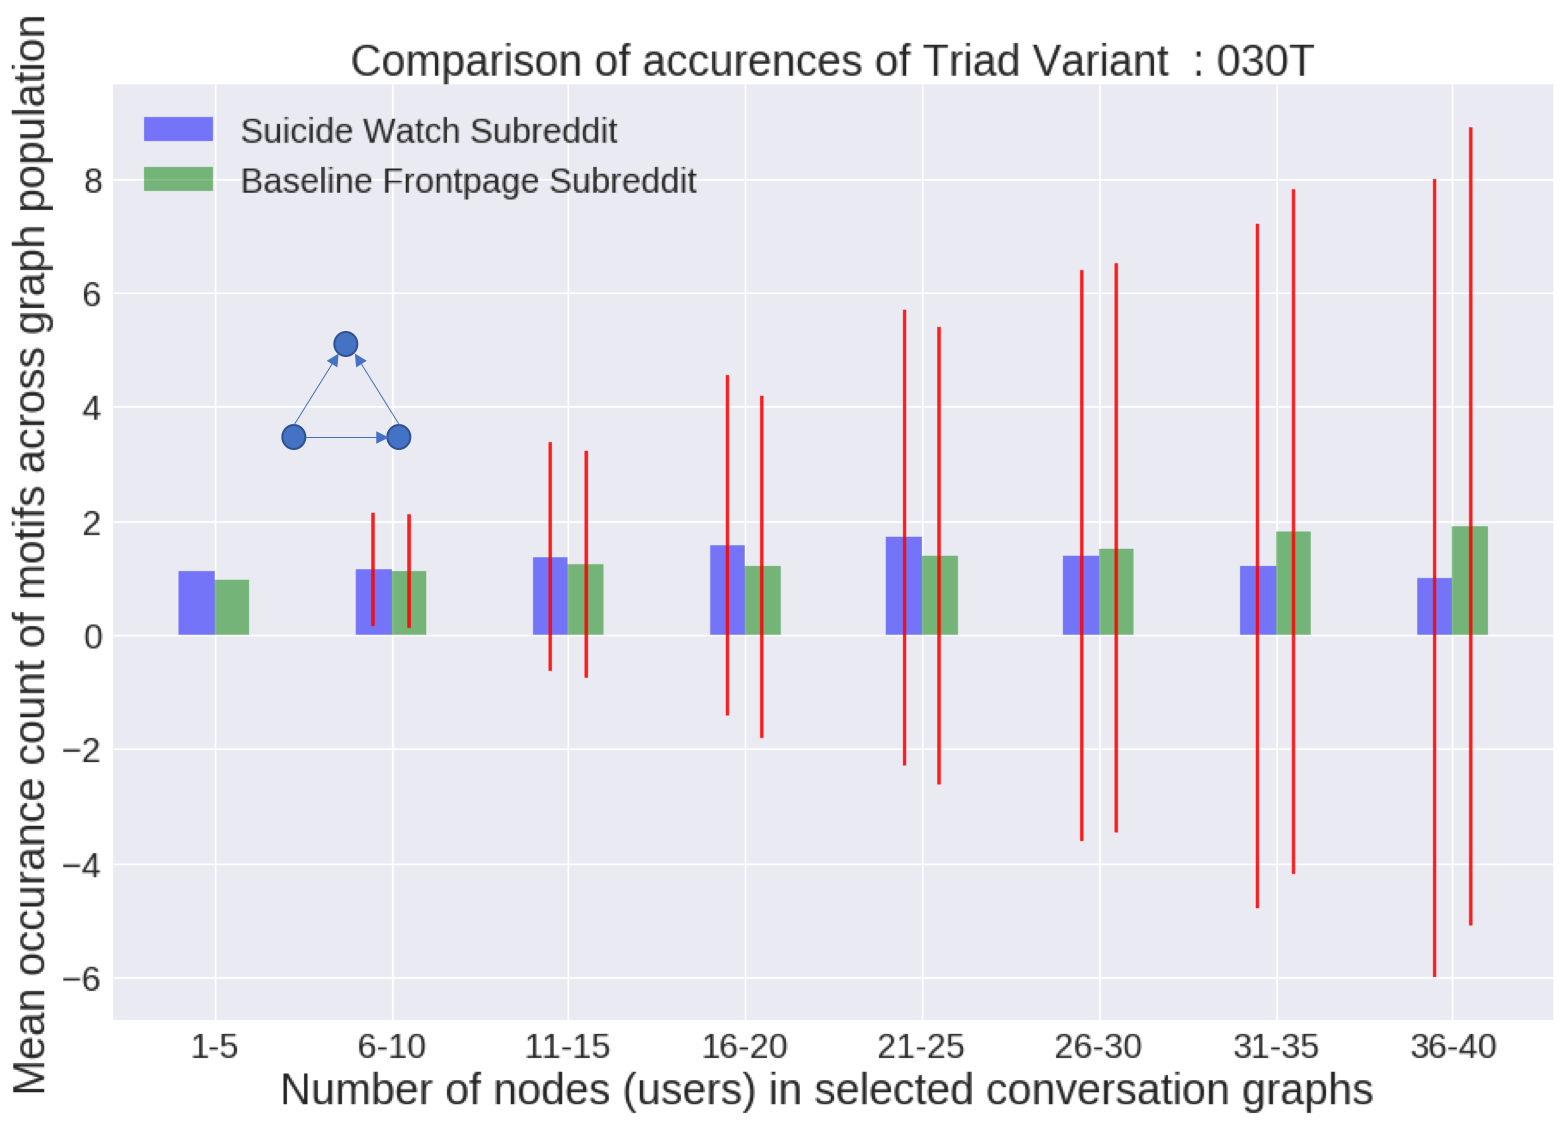
\includegraphics[width=0.33\textwidth, height = 4.5cm ]{030T}
        \label{fig:030T}
    }
    
    \subfloat[]{
        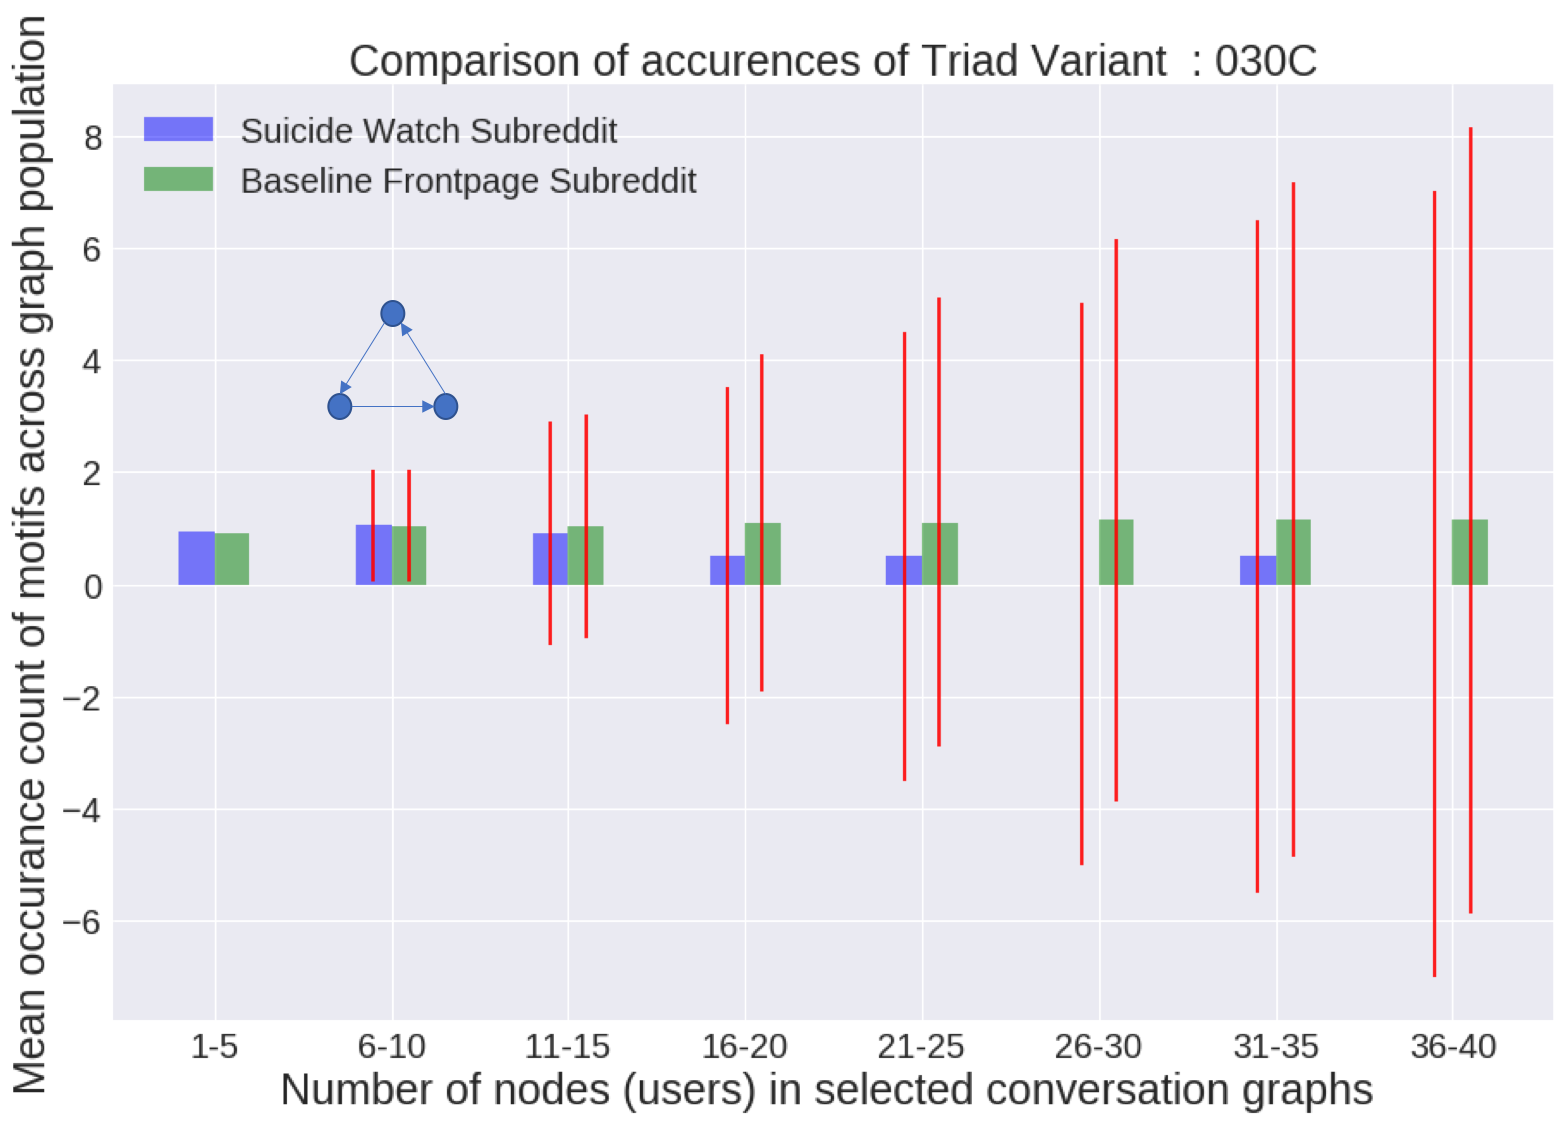
\includegraphics[width=0.33\textwidth, height = 4.5cm ]{030C}
        \label{fig:030C}
    }
    \subfloat[]{
        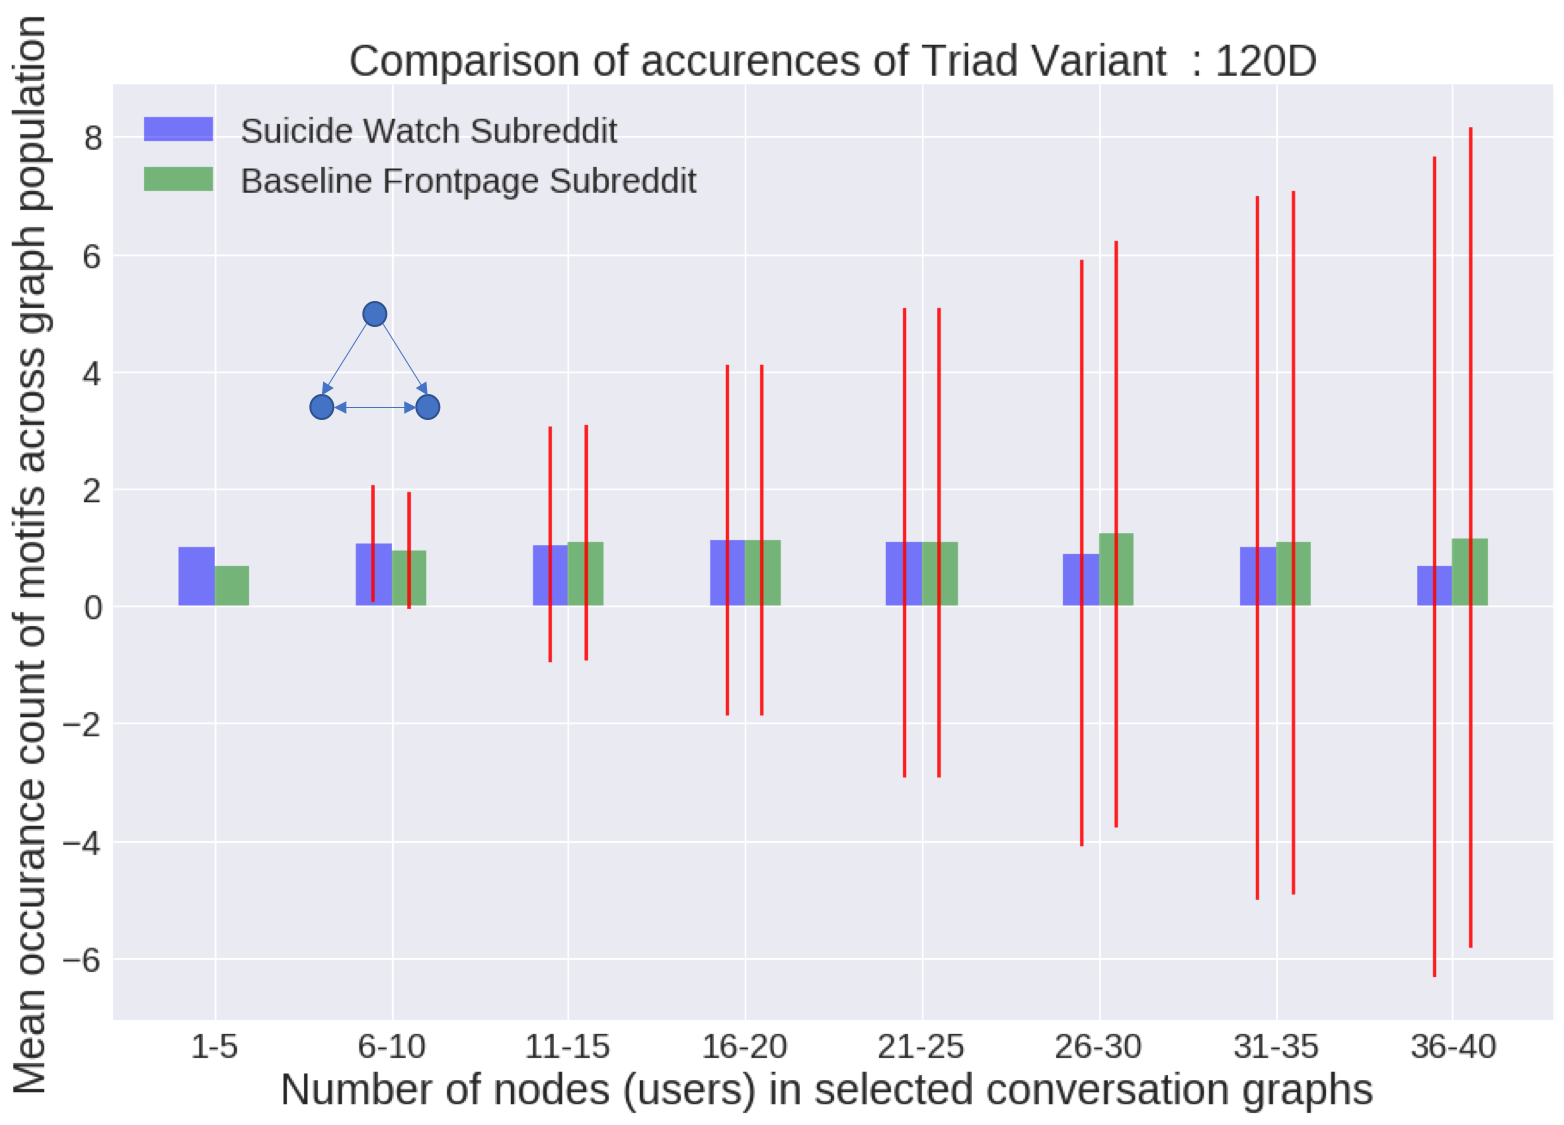
\includegraphics[width=0.33\textwidth, height = 4.5cm ]{120D}
        \label{fig:120D}
    }
    \subfloat[]{
        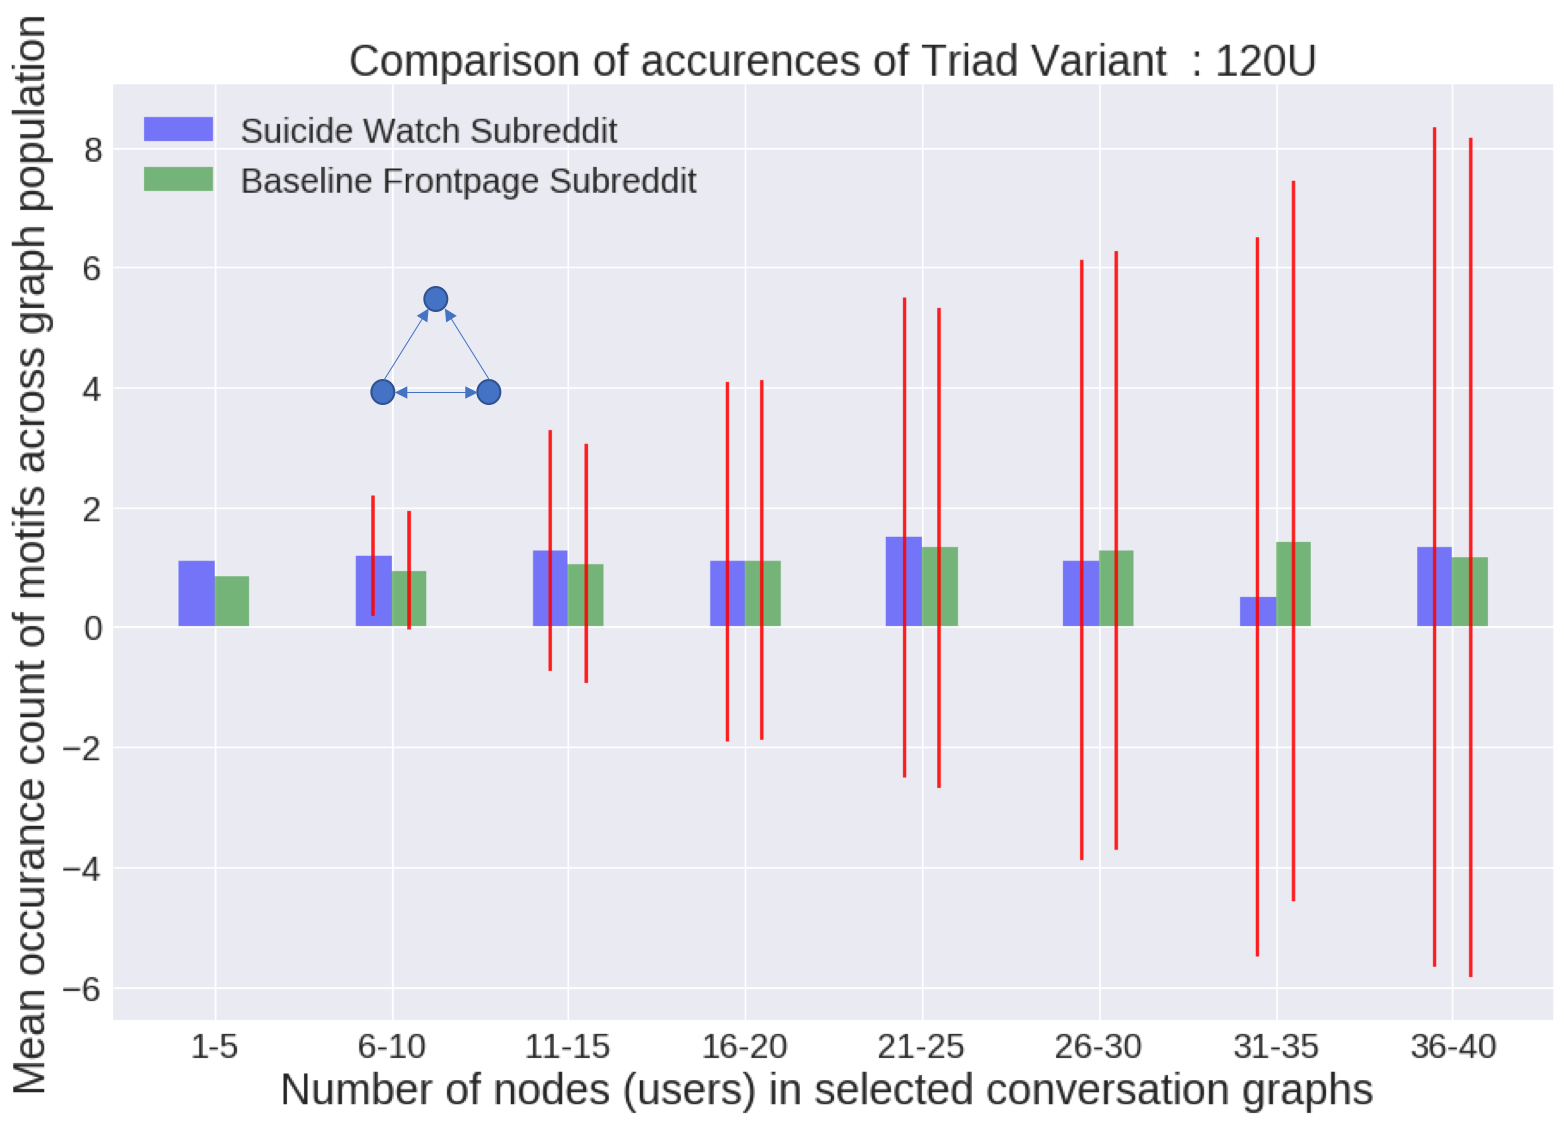
\includegraphics[width=0.3\textwidth, height = 4.5cm ]{120U}
        \label{fig:120U}
    }
    
    \subfloat[]{
        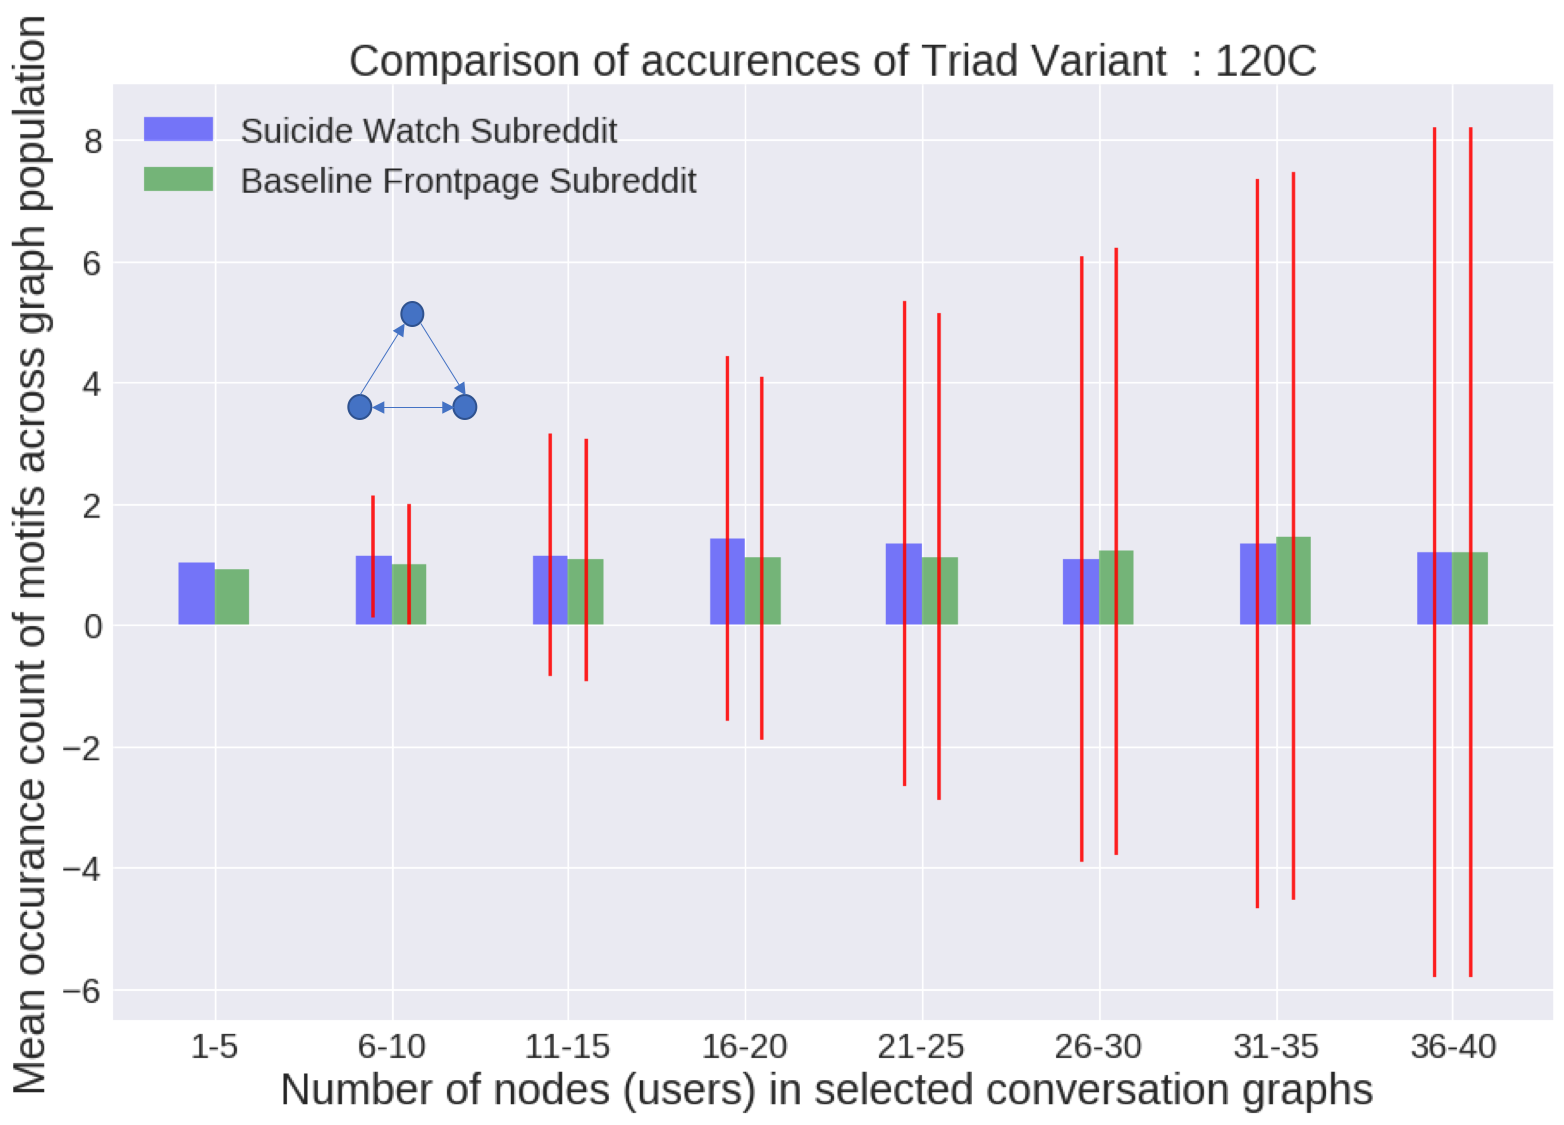
\includegraphics[width=0.33\textwidth, height = 4.5cm ]{120C}
        \label{fig:120C}
    }
    \subfloat[]{
        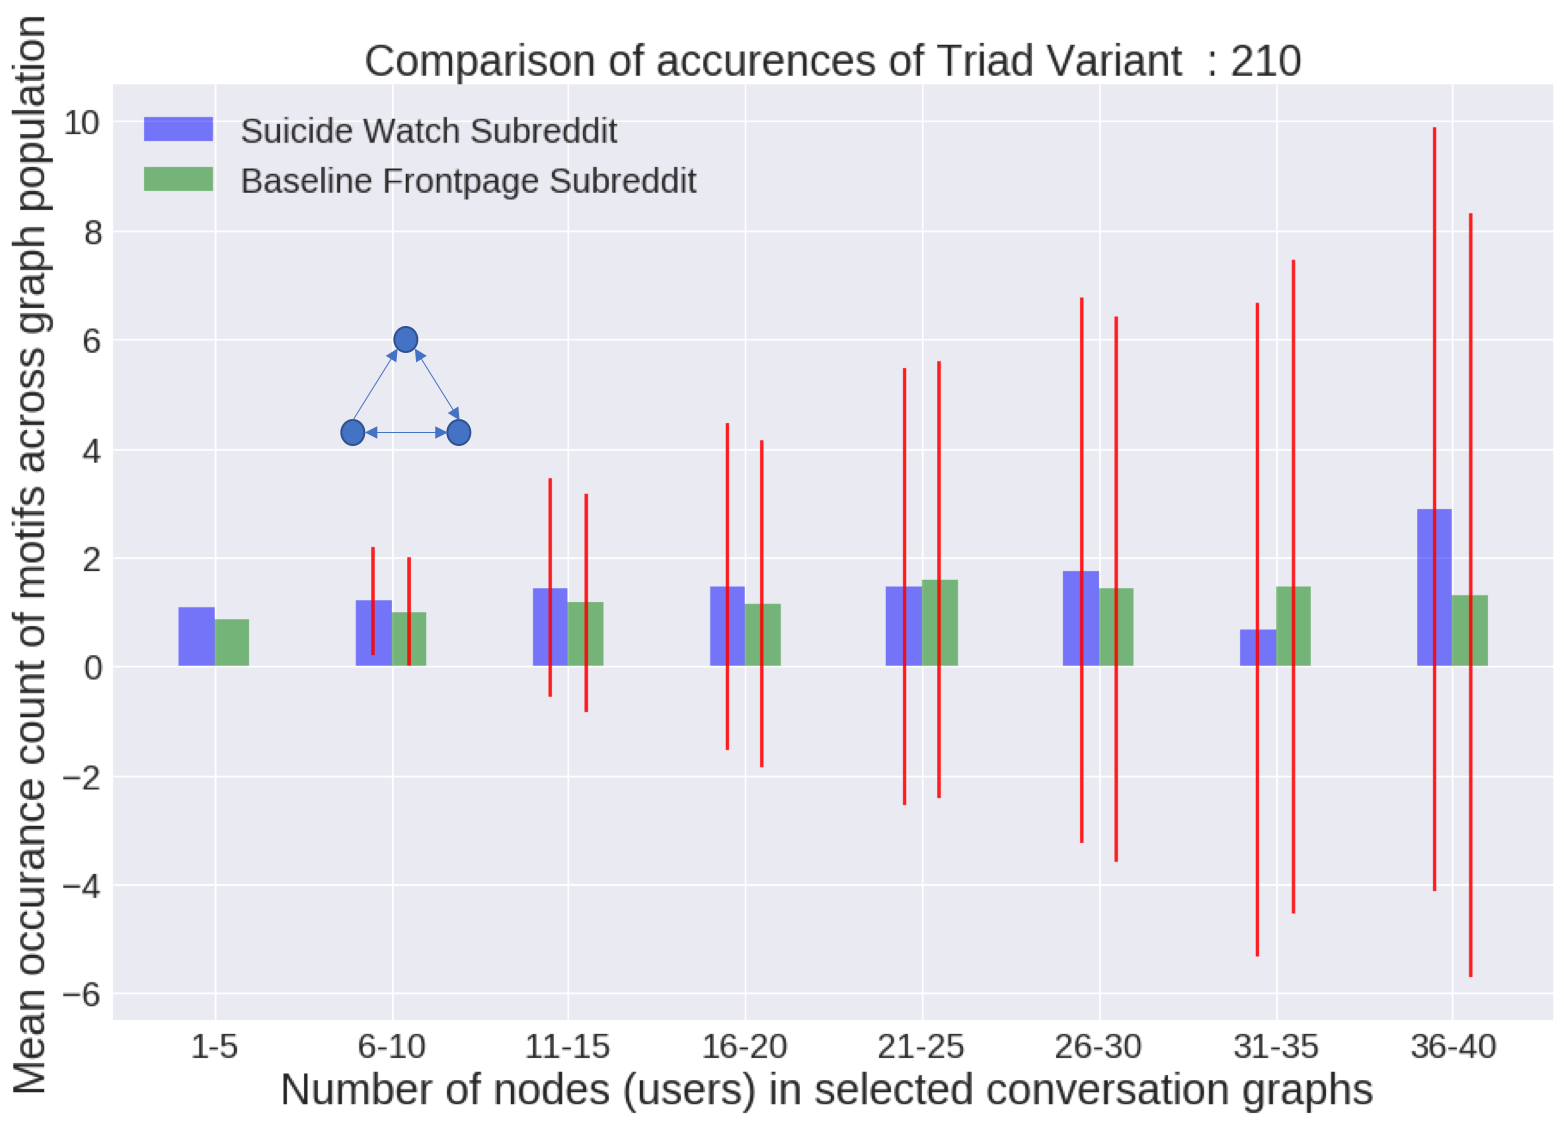
\includegraphics[width=0.33\textwidth, height = 4.5cm ]{210}
        \label{fig:210}
    }
    \subfloat[]{
        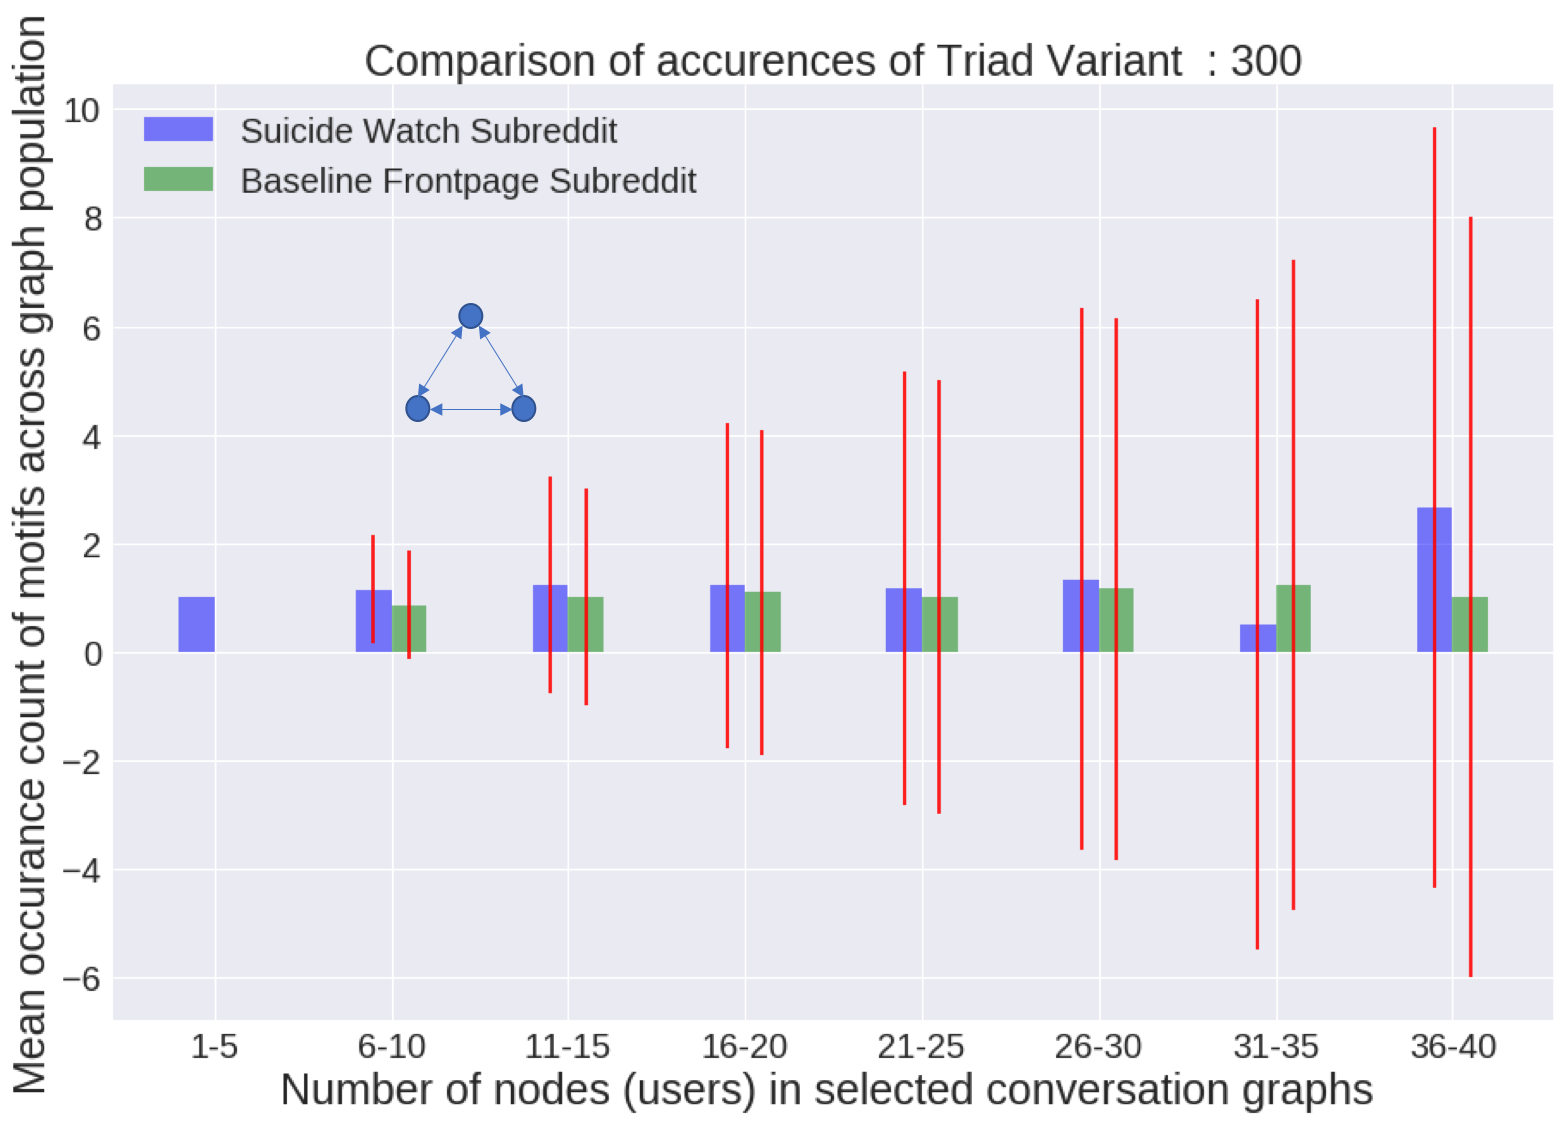
\includegraphics[width=0.33\textwidth, height = 4.5cm ]{300}
        \label{fig:300}
    }
    
    \label{fig:MotifOccurance}
    \vspace{-0.4cm}
    \caption{ The figure shows comparison of occurrence ratios of 9 insignificant motifs. Blue traces are for Suicide watch and Green traces are for Baseline Front page threads}
    \vspace{-0.4cm}
\end{figure*}





\subsection{}
Replication of quantification of the topological metrics for twitter conversations for suicidal ideation and comparison with baseline threads. There are 5k threads for suicidal ideation and 6k for baseline. The baseline threads deal with discussion around westminster and manchester terrorist attacks in the uk.

\begin{figure}[!h]
    \centering
    % \hspace*{-5mm}
    \subfloat[]{
        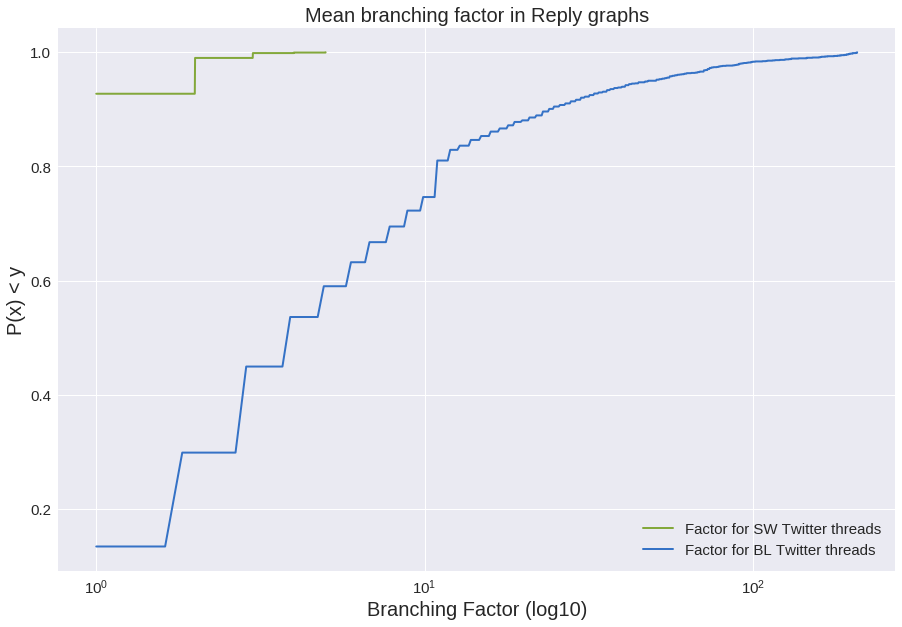
\includegraphics[width=0.4\textwidth, height = 5cm ]{Twitter_mean_Branching.png}
        \label{fig:TwitBranch} }	
    \subfloat[]{
        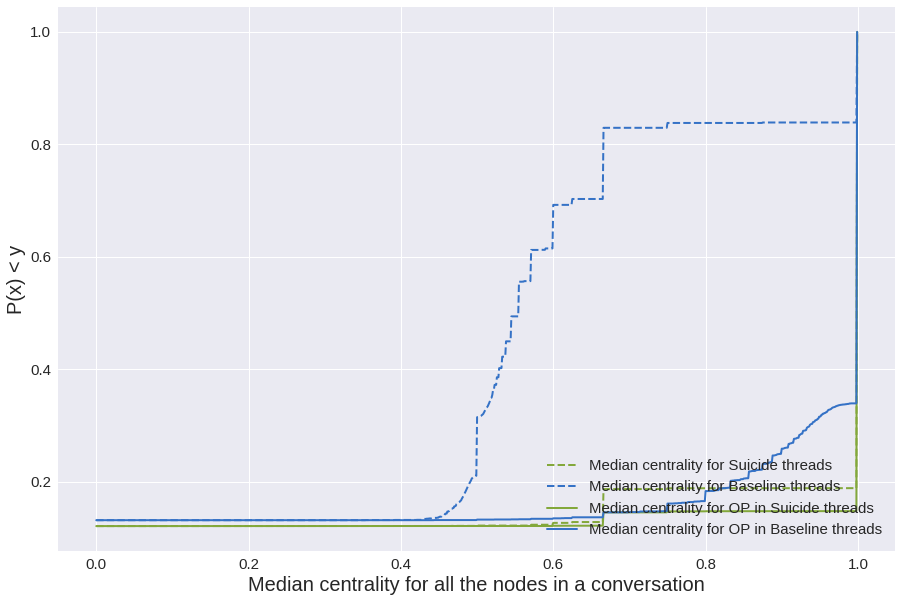
\includegraphics[width=0.4\linewidth, height = 5cm ]{Twitter_median_centrality.png}
        \label{fig:TwitCentrality}
    }
    
    
    \subfloat[]{
        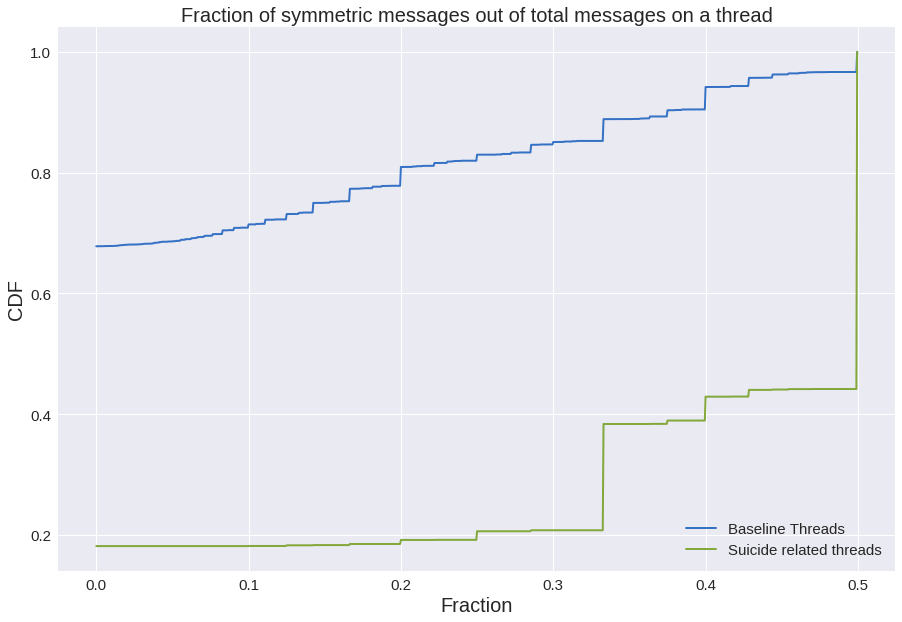
\includegraphics[width=0.4\textwidth, height = 5cm ]{Twitter_sym_messages.png}
        \label{fig:TwitSymMessages}
    }
    \subfloat[]{
        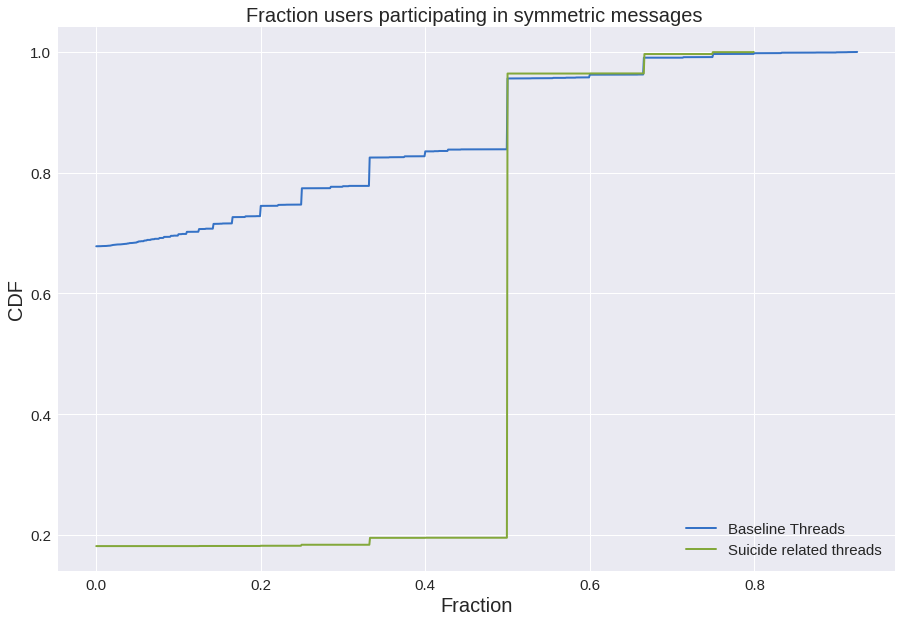
\includegraphics[width=0.4\linewidth, height = 5cm ]{Twitter_sym_users.png}
        \label{fig:TwitSynUsers}
    }
    
    \subfloat[]{
        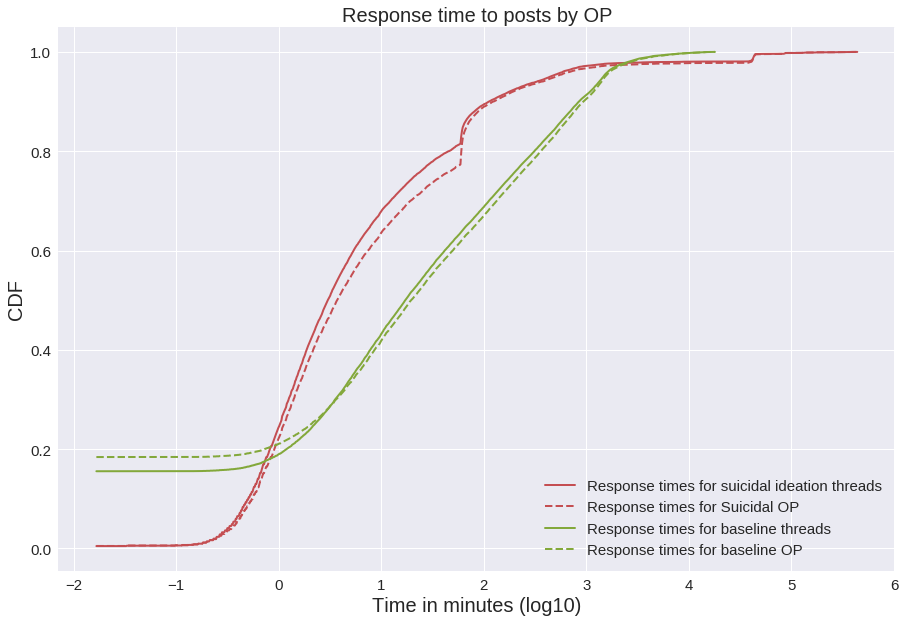
\includegraphics[width=0.4\linewidth, height = 5cm ]{Twitter_urgancy.png}
        \label{fig:TwitUrgency}
    }
    \caption{\textsl{ Fig \ref{fig:TwitBranch} shows the branching factor for twitter threads that talk about suicidal tendencies against baseline threads. Fig \ref{fig:TwitCentrality} shows the distribution of median centralities per thread, for both the twitter crawls. Fig \ref{fig:TwitSymMessages} shows Distribution of symmetric messages in reply graphs for both datasets. Fig \ref{fig:TwitSynUsers} shows the distributions for users participating in a symmetric conversation Fig \ref{fig:TwitUrgency} shows he dustribution of reply urgency for suicide threads against baseline. The suicide median reponse time for suicide threads is 3 min as compared to 18 mins for non-suicide threads}}
\end{figure}




\subsection{Network characteristics}
Figure \ref{fig:depthDist} shows the distribution of maximum depths across all Reply graphs for SW and Baseline subreddits. The SW threads depths have a median depth of 2 and mean of 4 compared to median depth of 2 for BL and a mean of 2.5. This shows that statistically the depths of Suicide watch and baseline graphs are quite similar.


\begin{figure}[!ht]
    \centering
    % \hspace*{-5mm}
    \subfloat[]{
        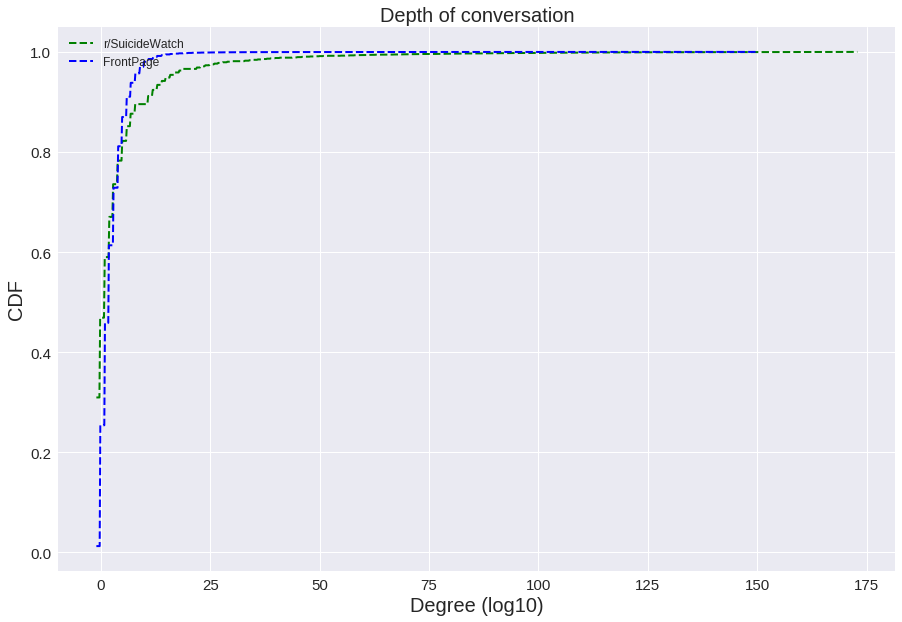
\includegraphics[width=0.4\textwidth, height = 5cm ]{DepthConversations.png}
        \label{fig:depthDist} }	
    \subfloat[]{
        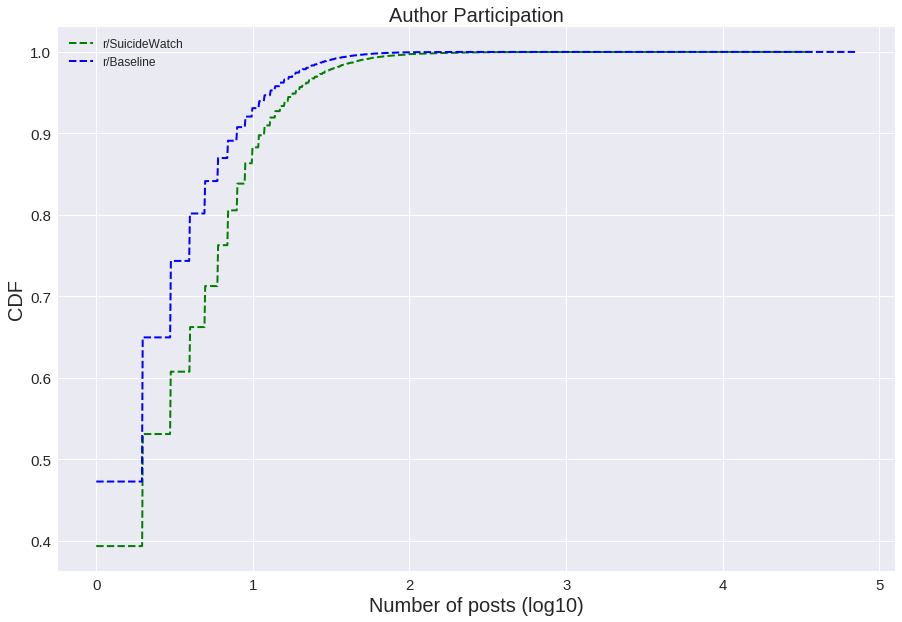
\includegraphics[width=0.4\linewidth, height = 5cm ]{AuthorParticipation.png}
        \label{fig:uniqAuthors}
    }
    
    
    \subfloat[]{
        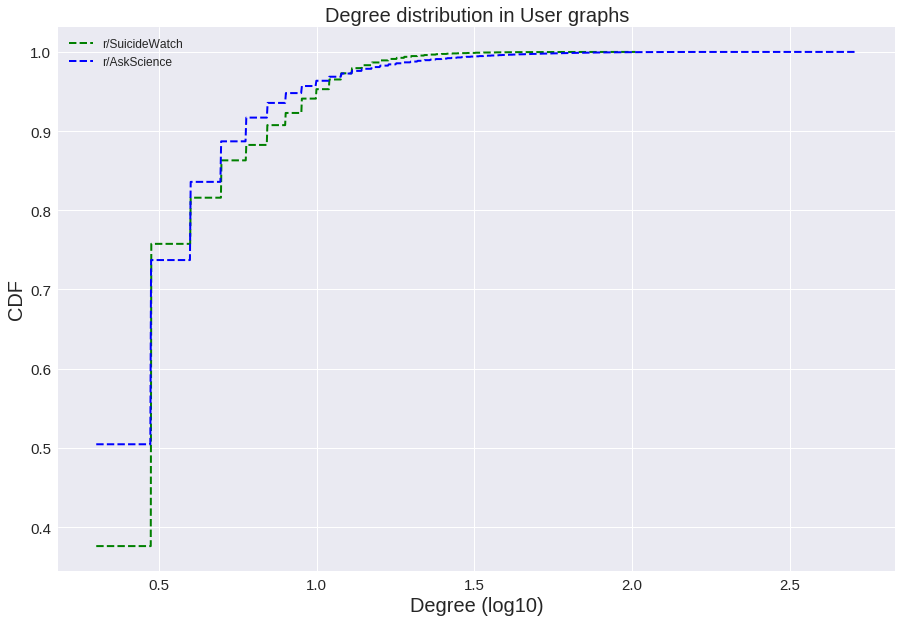
\includegraphics[width=0.4\textwidth, height = 5cm ]{degreeDistUgraph.png}
        \label{fig:degUgraph}
    }
    \subfloat[]{
        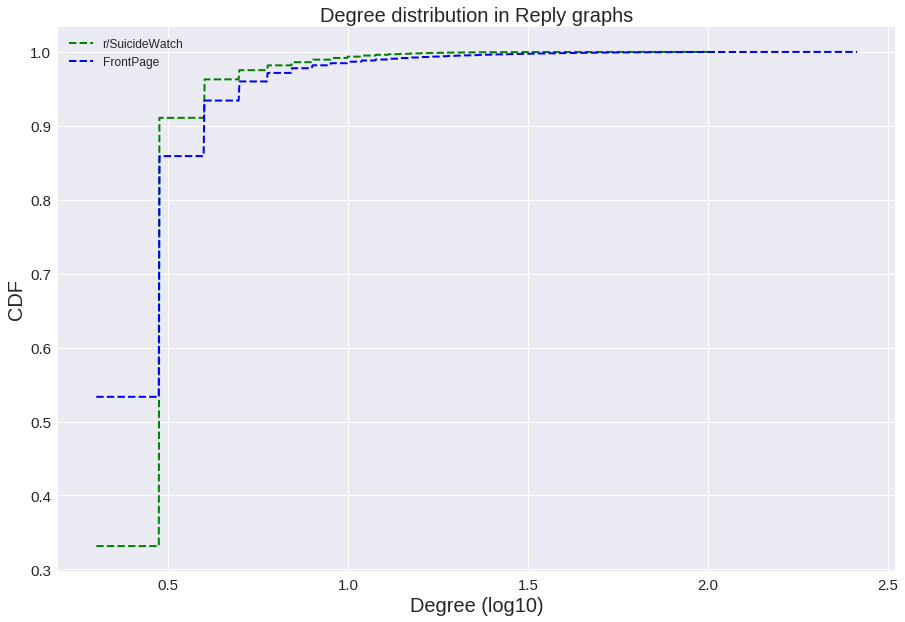
\includegraphics[width=0.4\linewidth, height = 5cm ]{degreeDistReplyGraph.png}
        \label{fig:degRgraph}
    }
    \caption{\textsl{ Fig \ref{fig:depthDist} shows the distribution of maximum depths of Reply Graphs for Subreddit r/SuicideWatch and the baseline Frontpage conversations. Fig \ref{fig:uniqAuthors} shows the distribution of unique authors per thread in the two datasets. Fig \ref{fig:degRgraph} shows Distribution of degrees for Reply Graphs,  r/SuicideWatch and FrontPage. Fig \ref{fig:degUgraph} shows the degree distributions for the reply graphs}}
\end{figure}

Figure\ref{fig:responseDist} shows the CDF for the number of responses a Root post gets on a thread across the whole dataset. 
\begin{figure}[!h]
    \centering
    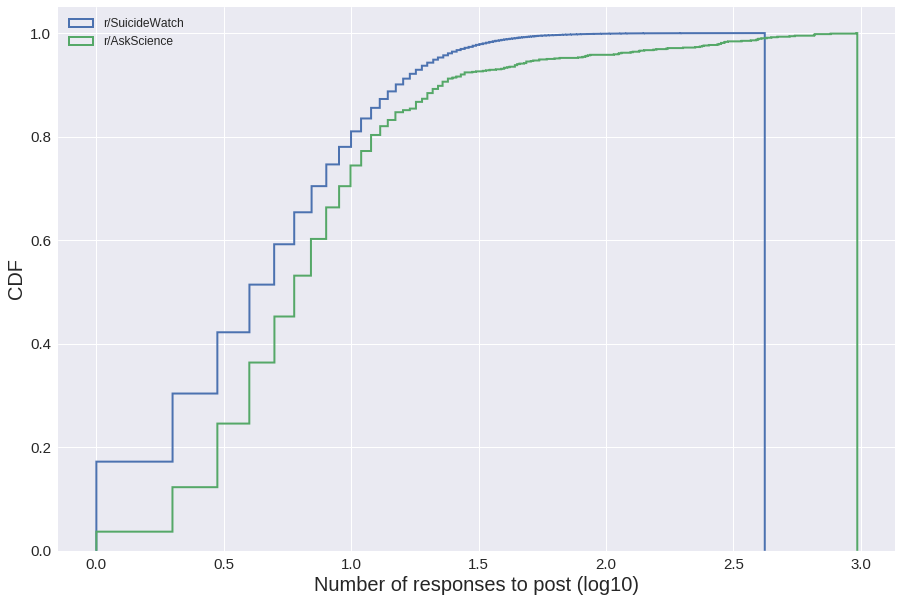
\includegraphics[width=0.4\linewidth]{responseDistSW}
    \caption{\textsl{ Distribution of responses per thread on Subreddits r/SuicideWatch and Frontpage }}
    \label{fig:responseDist}
\end{figure}
Figure \ref{fig:responseDist} shows the CDF for number of comments per thread across the r/SuicideWatch subreddit dataset and the crawled frontpage subreddit. 
